\documentclass[poster]{polytech/polytech}
\let\oldtabular=\tabular
\def\tabular{\scriptsize\oldtabular}


% LISEZ LE MODE D'EMPLOI POUR L'INTEGRALITE DES CONSIGNES

% on ajoute ici des packages supplémentaires
% Attention : il peut y avoir des incompatibilités avec la classe de document

\usepackage{lipsum} %permet de générer du texte
\usepackage{amsmath}
\usepackage{listings}
\usepackage{pdfpages}

% on indique le département concerné (di)
\schooldepartment{di}
% on indique le type de projet concerné (prd)
\typereport{prd}
% on indique l'année en cours
\reportyear{2015-2016}

% on donne un titre au travail (sans dépasser 2 lignes à l'affichage)
\title{Application d'aide à l'interaction homme/machine pour les personnes handicapées}
% on peut donner un sous titre (sans dépasser 2 lignes à l'affichage) mais ce n'est pas nécessaire
%\subtitle{Il peut y avoir un sous titre mais ce n'est pas obligatoire}
% on peut donner un logo illustrant le projet (hauteur d'affichage 4cm) mais ce n'est pas nécessaire
%\reportlogo{polytech/modeemploi}

% on indique les contributeurs à ce rapport

% Le(s) étudiant(s) aux formats suivants :
% \student{Prénom}{Nom}{Mail}
% \student[Année d'études]{Prénom}{Nom}{Mail}
\student[DI5]{Florian}{Tissier}{florian.tissier@etu.univ-tours.fr}
% Le(s) superviseur(s) académique (ou encadrant(s)) aux format suivants :
% \academicsupervisor{Prénom}{Nom}{mail}
% \academicsupervisor[Affiliation]{Prénom}{Nom}{mail}
\academicsupervisor[Département infomatique]{Mohamed}{Slimane}{mohamed.slimane@univ-tours.fr}
\academicsupervisor[Département infomatique]{Donatello}{Conte}{donetello.conte@univ-tours.fr}
% Le(s) tuteur(s) entreprise aux formats suivants :
% \companysupervisor{Prénom}{Nom}{Mail}
% \companysupervisor[Fonction]{Prénom}{Nom}{Mail}
% L'entreprise aux formats suivants :
%	\company{Nom de l'entreprise}{Adresse}{URL du site web}
% \company[logo entreprise]{Nom de l'entreprise}{Adresse}{URL du site web}
% S'il est indiqué le logo de l'entreprise s'affichera sur une hauteur de 1cm
% Attention : pour que les tuteurs entreprise s'affichent, l'entreprise doit être définie
%\company[polytech/polytech]{Laboratoire Informatique}{64 avenue Jean Portalis\\37200 Tours}{http://li.univ-tours.fr}
%\company{Laboratoire Informatique}{64 avenue Jean Portalis, 37200 Tours}{li.univ-tours.fr}


% On indique les mots clés avec \motcle{mot clé} en français et \keyword{keyword} en anglais
% Le résumé significatif et descriptif du contenu du rapport en 5 à 10 lignes se spécifie par \resume{...} en français et \abstract{...} en anglais
% Attention : tout doit tenir sur la dernière page
\resume{Dans le cadre de ce projet, j'ai pour mission de réaliser une application, destinée aux personnes handicapées, qui permettra de reconnaître leurs émotions et de réaliser certaines actions en conséquences (ex: changement de couleur de la lumière).\\
Dans la partie Recherche de ce projet, j'ai réalisé un état de l'art sur les différentes techniques permettant de reconnaître des émotions (filtres de Gabor, composantes pseudo-Haar,...) et sur comment construire un système de reconnaissance faciale d'expressions fiable et performant. Je me suis également documenté sur une nouvelle approche permettant de représenter des émotions sur un espace fini via un modèle probabiliste.}
% chaque mot clé ou groupe de mots clés est défini via la commande \motcle en français
\motcle{détection}
\motcle{émotion}
\motcle{filtres de Gabor}
\motcle{composantes pseudo-Haar}
\motcle{reconnaissance facial d'expression}
\motcle{FACS}
\motcle{bases de données de visages}
\motcle{modèle probabiliste}

% résumé en anglais
\abstract{During this project, I have the mission to realize an application, for disabled people, which will recognize their emotions and do specifics actions in consequences (e.g: change the color of the lights).\\
In the Research part of this project, I carried out a state of the art on the different technics allowing emotion recognition (Gabor filters, Haar-like features,...) and on how to build a reliable and efficient facial expression recognition system. I also documented myself about a new way that allows us to represent emotion on a finite space via a probabilistic model.}

% chaque mot clé ou groupe de mots clés est défini via la commande \keyword en anglais
% Attention : il n'y a pas forcément une traduction directe entre les mots clés et les keywords
\keyword{detection}
\keyword{emotion}
\keyword{Gabor filters}
\keyword{Haar-like features}
\keyword{facial expression recognition}
\keyword{FACS}
\keyword{faces databases}
\keyword{probabilistic model}


\bibliography{biblio}

\posterblock{Objectif}{
Repérer le visage d'une personne handicapée grâce à une caméra puis analyser son émotion actuelle.\\
En fonction de l'émotion récupérée, une action spécifique sera réalisée (ex: changement de couleur de la lumière). 
}{images/ptz.png}{}
\posterblock{Première approche}{
Utilisation de normes de description des mouvements faciaux, telle que la norme \textbf{FACS}, qui permet de définir 7 émotions (neutre, joie, tristesse, peur, surprise, colère et dégoût) en terme d'\textbf{Action Units} représentant des mouvements faciaux.\\
Approche de moins en moins adaptée aux problèmes d'aujourd'hui.
}{images/AU.png}{}
\posterblock{Nouvelle approche}{
Via un modèle probabiliste, il est possible de représenter les émotions sur un espace fini en 2 dimensions\\
En fonction de la position d'un point sur cet espace, on peut donc en déduire l'émotion associée.
}{images/ck2.jpg}{}

% le document commence ici
\begin{document}

% on commence par générer la page de titre, la liste des intervenants, les tables des matières, figures, tables, listings
\maketitle


% Le chapitre d'introduction générale n'est souvent pas numéroté
% La commande \unnumberedchapter fonctionne de façon identique à \chapter mais produit un chapitre non numéroté présent dans la table des matières (à la différence de \chapter*)
% Attention : un chapitre sans numéro (et ses sections) ne peu(ven)t pas être référencé(s) dans le document (\label, \ref)
\unnumberedchapter[Introduction]{Introduction}
L'interaction entre les hommes et les machines a toujours été un enjeu de taille. Arriver à faire communiquer un ordinateur avec un être humain est un défi de tous les jours et est de plus en plus présent dans notre quotidien. Nous pouvons par exemple citer \textit{Siri} d'Apple qui permet de communiquer avec son smartphone simplement en parlant.\\ 
C'est dans cette optique de facilitation du quotidien grâce à l'interaction avec une machine que ce projet prend place.\\
\\
Le Projet de Recherche et Développement (anciennement Projet de Fin d'Études) est un projet se déroulant durant toute la 5ème année de master ingénieur au sein de l'école Polytech Tours. Ce rapport va présenter les travaux que j'ai effectué durant toute la durée de ce projet.\\
\\
Ce rapport va donc se diviser en deux grandes parties: tout d'abord la partie Recherche qui va contenir le cahier des charges du projet, l'état de l'art en matière de reconnaissance faciale d'émotions ainsi que toutes les bases théoriques dont j'aurais besoin par la suite.\\
La deuxième partie est la partie Développement qui va se concentrer sur les différentes étapes du développement de cette application d'aide aux personnes handicapées.\\
\\
Dans la partie Recherche de ce rapport, après avoir défini le cahier des charges, je vais vous présenter les sept émotions universelles ainsi que deux normes majeures permettant de définir les mouvements du visages qui composent une expression.\\
Je vous présenterai ensuite un état de l'art en matière de reconnaissance faciale d'expression, notamment les différentes techniques permettant de capturer un visage et de reconnaître une émotion, tout d'abord en 3D puis en 2D, ainsi que les avantages et inconvénients de chacune de ces techniques. Dans chacune de ces étapes, je présenterai l'état de l'art actuelle en terme de matériel, de méthodes et également de base de données disponibles. \\
Je continuerai ensuite en présentant les différentes étapes nécessaires à la construction d'un système de reconnaissance faciale d'émotions performant et efficace.\\
Je définirai ensuite les spécifications de l'application ainsi que les choix qui ont permit cette définition.\\
Je conclurai par un planning prévisionnel ainsi que par les méthodologies et les outils de suivi utilisés durant ce projet.\\
\\
Dans la partie Développement, je présenterai, dans un premier chapitre, les modifications qui ont été identifiées (notamment grâce à un rendez vous avec Giuseppe Boccignone) et qui vont nous permettre de modifier le programme de Vitale et al. pour l'adapter à notre problématique.\\
J'expliquerai ensuite dans un second chapitre comment j'ai réalisé ces modifications.\\
Durant la phase d'identification des modifications, j'ai également dû rédiger un article scientifique, à propos de mes travaux réalisés durant ce projet, qui sera présenté, s'il est accepté, à la conférence Handicap 2016 organisé par l'IFRATH à Paris du 8 au 10 Juin 2016.\\
\\
Pour ce projet de recherche et développement, j'ai été encadré par Donatello CONTE et Mohamed SLIMANE.


\part{Recherche}
\label{part:part_recherche}

\chapter{Cahier des charges du projet}
\label{chap:chap_cdc}

\section{MOA}
\begin{itemize}
\item Donatello CONTE: Maître de conférence et enseignant chercheur en informatique à l'école Polytech Tours
\item Mohamed SLIMANE: Professeur des Universités et enseignant chercheur en informatique à l'école Polytech Tours
\end{itemize}

\section{MOE}
Florian TISSIER: élève en dernière année de master ingénieur en informatique à Polytech Tours

\section{Contexte et présentation}
Ce projet de recherche et développement prend place dans le cursus de dernière année de master ingénieur dispensé à l'école Polytech Tours.\\
\\
Monsieur Slimane étant membre d'une association s'occupant de personnes handicapées, il souhaitait pouvoir aider et faciliter la vie de ces derniers via un projet réalisé au sein de l'école.\\
Le but de ce projet de recherche et développement est de construire un système permettant, à partir d'un flux vidéo acquis grâce à une caméra, de détecter l'expression actuelle du visage d'une personne handicapée dans le but de réaliser certaines actions pouvant améliorer son bien être.

\section{Problématique et objectif}
Comment faciliter la vie quotidienne des personnes handicapées grâce à leurs émotions?\\
\\
L'objectif est de réaliser une application qui pourra détecter en temps réel les émotions d'une personne handicapée se trouvant dans une pièce à l'aide d'une caméra fixée à un mur de cette même pièce. La caméra devra être capable de bouger et de zoomer pour suivre le visage de la personne.\\
Une fois l'émotion détectée, des actions spécifiques devront être réalisées (ex: changement de la couleur de la lumière, lecture de musique douce...).

\section{Périmètre}
Ce projet se concentre principalement sur les personnes handicapées mais l'application qui résultera de ce projet pourra également être utilisé pour des personnes non handicapées.\\
L'application devra être fonctionnel dans n'importe quelle pièce d'une maison ou d'une structure spécialisée dans l'accueil de personnes handicapées.

\section{Description fonctionnelle}
Le projet se découpe en 2 fonctions principales:
\begin{itemize}
\item Repérer le visage
\item Reconnaître l'expression\\
\end{itemize}

Chacune de ces fonctions se décomposent en plusieurs sous-fonctions.

\subsection{Repérer le visage}
Cette première fonction principale va permettre de trouver le visage d'une personne, de le suivre et de zoomer dessus.\\
Les sous-fonctions suivantes seront donc nécessaires:
\begin{itemize}
\item Un algorithme de détection de visage dans une image
\item Un algorithme de suivi de visage
\item Un algorithme de zoom\\
\end{itemize}

Vous trouverez ci-après un descriptif plus précis de chacune de ces sous-fonctions.

\begin{tabular}{|l|p{12.5cm}|}
   \hline
   \multicolumn{2}{|l|}{\textbf{Fonction F1: Repérer le visage/Détection du visage}} \\
   \hline
   Objectif &Détecter un visage dans un environnement quelconque.\\
   \hline
   Description &En analysant les frames d'un flux vidéo, cet algorithme nous renverra la position d'un cadre entourant le visage trouvé.\\
   \hline
   Contraintes &Cet algorithme doit être rapide. \\
   \hline
   Niveau de priorité &Haute \\
   \hline
\end{tabular}

\begin{tabular}{|l|p{12.5cm}|}
   \hline
   \multicolumn{2}{|l|}{\textbf{Fonction F2: Repérer le visage/Suivi du visage}} \\
   \hline
   Objectif &Suivre le visage entre plusieurs frames d'un flux vidéo dans le but de ne pas le perdre. \\
   \hline
   Description &En comparant 2 frames consécutives d'un flux vidéo, l'algorithme devra nous dire le déplacement du visage pour pouvoir le suivre avec la caméra. Il devra également être capable de faire le suivi si jamais le visage se retrouve occulté pendant quelques secondes. \\
   \hline
   Contraintes &Éviter le plus possible l'accumulation d'erreur de précision pouvant amener à la perte du visage. \\
   \hline
   Niveau de priorité &Haute \\
   \hline
\end{tabular}

\begin{tabular}{|l|p{12.5cm}|}
   \hline
   \multicolumn{2}{|l|}{\textbf{Fonction F3: Repérer le visage/Zoom}} \\
   \hline
   Objectif &Zoomer sur une zone de l'image. \\
   \hline
   Description &L'algorithme devra pouvoir zoomer sur le cadre contenant le visage renvoyé par la sous-fonction F1. \\
   \hline
   Contraintes &Disposer d'une caméra ayant la possibilité de zoomer. \\
   \hline
   Niveau de priorité &Moyenne \\
   \hline
\end{tabular}
\newpage
\subsection{Reconnaître l'expression}
Cette deuxième fonction principale va permettre d'identifier l'expression faciale de la personne.\\
Les sous-fonctions suivantes seront donc nécessaires:
\begin{itemize}
\item Un algorithme d'apprentissage
\item Un algorithme d'extraction des points clés (\textit{features}) du visage
\item Un algorithme de classification\\
\end{itemize}

Vous trouverez ci-après un descriptif plus précis de chacune de ces sous-fonctions.

\begin{tabular}{|l|p{12.5cm}|}
   \hline
   \multicolumn{2}{|l|}{\textbf{Fonction F4: Reconnaître l'expression/Apprentissage}} \\
   \hline
   Objectif &Apprendre au système à classifier les expressions en fonction d'une base d'apprentissage.\\
   \hline
   Description &Pour chaque élément dans la base d'apprentissage, une émotion lui sera associé. Cela va permettre au système d'apprendre à quelle expression du visage appartient une émotion.\\
   \hline
   Contraintes &La base d'apprentissage doit être assez fournie et pertinente pour permettre un apprentissage performant. \\
   \hline
   Niveau de priorité &Haute \\
   \hline
\end{tabular}

\begin{tabular}{|l|p{12.5cm}|}
   \hline
   \multicolumn{2}{|l|}{\textbf{Fonction F5: Reconnaître l'expression/Extraction des \textit{features} du visage.}} \\
   \hline
   Objectif &Extraire les \textit{features} du visage pour pouvoir ensuite réaliser une classification. \\
   \hline
   Description &Cet algorithme devra extraire les \textit{features} du visage d'une personne se trouvant sur une frame d'un flux vidéo. Les \textit{features} d'un visage sont par exemple le coin des yeux, la position de la pupille, les coins de la bouche, le nez, les joues... Les positions des \textit{features} retournées permettront la classification. \\
   \hline
   Contraintes & \\
   \hline
   Niveau de priorité &Haute \\
   \hline
\end{tabular}

\begin{tabular}{|l|p{12.5cm}|}
   \hline
   \multicolumn{2}{|l|}{\textbf{Fonction F6: Reconnaître l'expression/Classification}} \\
   \hline
   Objectif &Classifier l'expression du visage et retourner l'émotion associée. \\
   \hline
   Description &L'algorithme devra classifier l'expression du visage de la personne récupérée depuis un flux vidéo, grâce aux positions des \textit{features}, en fonction de l'apprentissage qui aura été effectué précédemment. \\
   \hline
   Contraintes &Cet algorithme doit être rapide et fiable (au moins 90\% de reconnaissance). \\
   \hline
   Niveau de priorité &Haute \\
   \hline
\end{tabular}

\section{Budget}
Ce projet ne dispose pas d'un budget précis.\\
Néanmoins en réalisant un état de l'art des matériels disponibles à notre projet, nous avons décidé de choisir une caméra ne dépassant pas les 500€.

\section{Délai}
La partie recherche devra être fini pour le 15 janvier 2016 et la partie développement (et donc le projet complet) devra être fini pour la fin du second semestre, c'est-à-dire fin mars.

\section{Livrable}
Le livrable de ce projet correspondra en une application Matlab qui réalisera la phase d'apprentissage et la classification des émotions.

\chapter{Émotions universelles et \mbox{mouvements} du visage}
\label{chap:chap_emotions}

Ce chapitre va me permettre d'introduire les notions nécessaires à la décomposition et donc à la reconnaissance d'une expression faciale et de son émotion associée.\\
Pour un simple sourire, nous utilisons une vingtaine de muscles (les muscles zygomatiques), il ne peut donc pas être décrit par un seul mouvement du visage mais plusieurs. C'est exactement la même chose pour une expression, on ne la reconnaît que grâce à l'ensemble des mouvements faciaux qui la composent.\\
C'est sur ce principe qu'ont été créé les deux normes de description des mouvements du visage que je vais vous présenter: le FACS et MPEG-4.\\
L'utilisation de l'une ou l'autre de ces normes permet de définir entièrement le spectre des mouvements rentrant en jeu dans n'importe quelle émotion.\\
\\
Mais tout d'abord, je vais vous introduire les sept émotions universelles qui seront utilisées tout au long de mon projet et donc de ce rapport.

\newpage
\section{Les 7 émotions universelles}
\label{sec:expr_uni}

A ce jour, il a été démontré qu'il existait 7 émotions qui partagent une expression universellement compréhensible.\\
On considère qu'une émotion possède une expression universelle si tout individu est capable d'exprimer cette émotion et est également capable de la reconnaître et de l'interpréter chez autrui.\\
Les sept émotions universelles sont donc les suivantes:
\begin{itemize}
	\item la neutralité
	\item la joie
	\item la tristesse
	\item la colère
	\item la peur
	\item la surprise
	\item le dégoût
\end{itemize}

C'est Charles Darwin qui, en 1872 dans son livre \cite{darwin}, a introduit cette idée d'émotions universelles entre les hommes mais également entre différentes espèces. Il a observé que les hommes et les animaux partagent des émotions comprises par tous et qui sont nécessaires à leur survie.\\
\\
Mais ce n'est qu'en 1971 que le psychologue Paul Ekman, après un voyage en Papouasie-Nouvelle-Guinée, a confirmé les théories de Darwin. Dans son article \cite{ekman} écrit avec la participation de Wallace Fielsen, il définit les 7 émotions universelles citées plus haut.\\

\section{Le FACS}
\label{sec:facs}

En 1978, Ekman et Fielsen publie \cite{ekman2} et apporte une nouvelle pierre à l'édifice en définissant un système de codification manuelle des expressions du visage: le \textbf{Facial Action Coding System} (FACS).\\
Ce système décompose tous les mouvements du visage en 46 \textbf{Action Units} (AU), chacune décrivant la contraction ou la décontraction d'un ou plusieurs muscles du visage. La \autoref{ex_au} représente certaines de ces AUs.\\

\begin{Figure}{ex_au}{Exemples d'AUs}
 \pgfimage{images/AU.png}
\end{Figure}

La composition de plusieurs AU permet donc de décrire une expression et donc de reconnaître une émotion. Par exemple, un sourire et donc l'émotion de la joie est composé des AUs 6 (remontée des joues) et 12 (étirement du coin des lèvres).\\
La tristesse quand à elle va être composée des AUs 1, 4 et 15 et la colère des AUs 4, 5, 7 et 23.\\
N'importe quelle expression du visage peut donc être représentée par une combinaison d'AU, ce qui fait de FACS le système le plus utilisé par les psychologues ainsi que par les personnes travaillant sur la reconnaissance faciale d'émotions.\\
\\
Le système \textbf{FACS} possède également un degré d'intensité allant de A à E et permettant de spécifier l'intensité d'une AU :
\begin{itemize}
	\item A : Très Faible
	\item B : Minime
	\item C : Moyen
	\item D : Sévère
	\item E : Maximum
\end{itemize}
La surprise peut donc être défini comme la combinaison des AUs 1, 2, 5B et 26.\\
\\
Enfin des ajouts ont été apportés à cette norme. 13 nouveaux AUs ont été ajoutées pour décrire le mouvement de la tête et 7 autres pour le mouvement des yeux.\\
Nous arrivons donc a un total de 66 AUs, chacune possédant 5 intensités, permettant de décrire les mouvements faciaux.\\
\\
Néanmoins, un autre système de codification fait concurrence au FACS et est également bien implanté dans le milieu de la reconnaissance d'émotions.

\section{La norme MPEG-4}
\label{sec:fapu}

La norme MPEG-4, qui est une norme de codage vidéo, dispose de son propre système permettant de normaliser les mouvements du visage et de reconnaître des expressions.\\
Pour cela, ce système défini des points clés du visage (\autoref{points_fapu}) appelés \textbf{Facial Features Points} (FFP) auxquels seront appliqués des mesures pour créer des distances entre ces FFP (\autoref{distance_fapu}) appelées \textbf{Facial Animation Parameter Units} (FAPU).\\
Ces FAPU vont servir à la description des mouvements musculaires appelés \textbf{Facial Action Parameters} (FAP, équivalent des AUs de la norme FACS). 68 FAPs sont recensés à ce jour, j'en ai regroupé quelques uns dans le tableau \autoref{tab:fap}.\\
Le descriptif complet de ces FAP se trouve dans le document à cette adresse \cite{urlfaps}, dans l'annexe numéro 1.

\begin{Table}{tab:fap}{Exemple de Facial Action Parameters}
	\begin{tabu}{|c|c|X[m]|}
		\hline
		Numéro &Nom &Description\\\hline
		3 &open\_ jaw &Déplacement vertical de la mâchoire (n'affecte pas l'ouverture de la bouche)\\\hline
		7 &stretch\_ r\_ cornerlip &Déplacement horizontal du coin droit de la lèvre intérieure\\\hline
		10 &raise\_ b\_ lip\_ lm  &Déplacement vertical du point médian entre le coin gauche et le bas de la lèvre intérieure\\\hline
		42 &lift\_ r\_ cheek &Déplacement vertical de la joue droite\\\hline
	\end{tabu}
\end{Table}

\begin{Figure}{points_fapu}{Quelques Facial Features Points utilisés par la norme MPEG-4}
 \pgfimage{images/points_fapu.png}
\end{Figure}

\begin{Figure}{distance_fapu}{Facial Animation Parameter Units utilisés par la norme MPEG-4}
 \pgfimage{images/distance_fapu.png}
\end{Figure}

Cependant, la norme de MPEG-4 est moins réaliste que FACS d'un point de vue musculaire.\\
Par exemple : l'AU 26 de FACS (« Jaw Drop ») décrit le mouvement d'abaissement du menton, cet abaissement est accompagné d'un abaissement de la lèvre inférieure. Or l'abaissement du menton de MPEG-4 (FAP 3 - open\_ jaw) ne décrit pas l'abaissement de la lèvre inférieure.\\
\\
Nous allons maintenant voir quelles technologies sont disponibles pour réaliser l'acquisition des images qui seront à traiter par la suite.

\chapter{État de l'art}
\label{chap:chap_sota}

Dans ce chapitre, je vais vous présenter l'état de l'art des systèmes et techniques existants permettant de faire de la reconnaissance facial d'émotion.\\
Mon projet se basant sur des images et vidéos en 2D, ce chapitre va principalement se concentrer sur les techniques d'acquisition et d'analyse d'images 2D.\\
Cependant, j'ai tout de même réalisé quelques recherches sur le matériel utilisé pour l'acquisition d'images en 3D ainsi que les bases de données disponibles et c'est donc par ces recherches que je vais entamer ce chapitre.

\newpage
\section{3D}
\label{sec:3d}

Comme je l'ai expliqué plus haut, mon projet, et donc mon système de reconnaissance, utilisera des images 2D mais j'ai tout de même mené quelques recherches sur les images en 3D également.\\
Je vais tout d'abord vous présenter les techniques utilisées pour acquérir des images en 3D. Je vous exposerai ensuite certains matériels déjà existant permettant de faire de la capture d'images 3D et utilisant les techniques que je vous aurais présenté précédemment. Je terminerai enfin cette section sur la 3D en vous introduisant les bases de données de visages les plus connues et les plus utilisées par les systèmes de reconnaissance faciale d'émotion en 3D.\\
Les informations que vous allez trouver dans cette section proviennent en majorité de l'article \cite{sota3d}.

\subsection{Techniques d'acquisition}
\label{subsec:tech}

\subsubsection{Reconstruction à partir d'une image}
\label{single_img_reconstruct}
Il est possible, à partir d'une image en 2D capturé par une caméra basique, d'obtenir une image en 3D.\\
La méthode la plus prometteuse est celle du \textbf{3D Morphable Model} (3DMM), qui consiste à apposer un visage en 3D (masque) sur l'image en 2D et de le modifier pour le faire correspondre avec l'image. Sont ensuite extraites les informations correspondant au masque modifié qui vont permettre de créer le visage de l'image en 3D.\\
La \autoref{3dmm} présente un exemple de visage 3D récupéré depuis une image 2D.\\
Cette technique est très pratique et répandue car elle ne nécessite pas de matériel au coût exorbitant, une simple caméra est nécessaire.

\begin{Figure}{3dmm}{Reconstruction d'un visage 2D (1) en 3D (2) grâce à la méthode 3DMM}
 \pgfimage{images/3dmm.png}
\end{Figure}

\subsubsection{Lumière structurée}
\label{struc_light}
Une autre technique, une des plus utilisé, est la technique de la lumière structurée.\\
Elle consiste à projeter plusieurs rais de lumière (visible ou infra-rouge) de longueur d'onde différente puis, à l'aide d'un capteur, de mesurer la déformation de ces rais de lumière pour construire le visage en 3D.\\
La \autoref{structured} montre un exemple de lumière structurée.\\
L'utilisation de cette technique requiert d'avoir un matériel spécifique contenant un émetteur et un récepteur, cet outil peut aller de quelques centaines d'euros pour les moins chère à plusieurs dizaines de milliers d'euros pour les plus performants.

\begin{Figure}{structured}{Exemple de lumière structurée}
 \pgfimage{images/structured.jpg}
\end{Figure}

\subsubsection{Stéréo photométrique}
\label{photo_stereo}
La technique de la stéréo photométrique consiste à prendre plusieurs photos d'un même objet avec un même appareil sous différentes illuminations (lumière venant de droite, lumière venant de devant ...). Pour obtenir un visage en 3D, il ne reste qu'à assembler les photos obtenues.\\
La \autoref{stereo_imgs} montre un exemple de reconstruction d'un objet grâce à la stéréo photométrique.\\
Cette technique requiert également un équipement coûteux et n'est donc pas accessible à tout le monde.

\begin{Figure}{stereo_imgs}{Exemple de reconstruction d'un objet grâce à la stéréo photométrique}
 \pgfimage{images/stereo_imgs.png}
\end{Figure}


\subsubsection{Stéréo multi-vue}
\label{multi_stereo}
C'est une technique très similaire à celle de la stéréo photométrique sauf qu'au lieu de prendre en photo un visage sous différentes illuminations, le visage est pris sous différents angles simultanément avec plusieurs appareils.\\
Cette technique requiert elle aussi un équipement spécifique coûteux.\\
\\
\\

\subsection{Dispositifs d'acquisition d'images}
\label{dispositif_acquisiton}
Plusieurs types de dispositifs différents existent à l'heure actuelle permettant de capturer des images en 3D. La plupart d'entre eux se basent sur les techniques présentées précédemment.\\
Je vais ici vous présenter les deux dispositifs les plus connus.

\subsubsection{Kinect}
\label{kinect}
Probablement la caméra 3D la plus connu du grand public : la Kinect de Microsoft.\\
Créer initialement pour créer une immersion plus poussée pour les jeux de la console XBox 360, elle a depuis été amélioré avec sa version XBox One et ne sert plus exclusivement qu'à jouer aux jeux vidéos.\\
Elle utilise la technique de la lumière structuré (infra-rouge dans ce cas) pour capturer les images en 3D de ce qu'elle filme.\\
La Kinect reste cependant une caméra 3D low-cost, de mauvaise qualité lorsqu'on le compare à d'autres dispositifs du même type, tel que celui que je vais présenter maintenant.

\begin{Figure}{kinect2}{Version 2 de la Kinect de Microsoft}
 \pgfimage{images/kinect2.png}
\end{Figure}

\subsubsection{Minolta Vivid 910}
\label{minolta}
Un autre dispositif très utilisé et utilisant lui aussi la technologie de la lumière structurée est le Minolta Vivid 910.\\
Un comparatif entre la qualité de Kinect et de Minolta est présenté en \autoref{kinectvsminolta}. On s'aperçoit très clairement du gouffre séparant ces deux dispositifs. Bien sûr le prix n'est pas le même, car nous passons de quelques centaines d'euros pour la Kinect à plusieurs dizaines de milliers d'euros pour le Minolta Vivid 910.

\begin{Figure}{img_minolta}{Minolta Vivid 910}
 \pgfimage{images/minolta.jpg}
\end{Figure}

\begin{Figure}{kinectvsminolta}{Comparatif de la qualité entre Kinect et Minolta}
 \pgfimage{images/kinectvsminolta.png}
\end{Figure}

\newpage
\subsection{Base de données de visages 3D}
\label{bdd3d}
Les dispositifs tels que le Minolta Vivid 910 présentées précédemment permettent également la création de bases de données de visage en 3D. Leurs grandes qualités permettent d'obtenir des images très précises, facilement exploitable.\\
Je vais maintenant vous présenter les bases de données les plus connues et pouvant être utilisée par la communauté scientifique.

\subsubsection{BU-3DFE}
Les premiers efforts pour récolter des données en 3D ont menés à la création de la base de données BU-3DFE (Binghamton University 3D Facial Expression \cite{bu3dfe_article}).\\
Les images contenues dans cette base sont statiques et ont été capturées par le dispositif 3dMD.\\
Elles se composent de 100 sujets âgés de 18 à 70 ans, dont 56\% de femmes, et appartenant à différentes ethnicités.\\
Chaque sujet réalise les 7 expressions basiques (cf \autoref{sec:expr_uni}) et chaque expression, sauf l'expression neutre, est réalisée suivant 4 niveaux d'intensités. Pour chaque sujet, il y a donc 25 images différentes, ce qui nous donne au total 2500 images dans cette base de données.\\
Un exemple de données contenues dans cette base sont présentés en \autoref{bu3dfe}.\\
Chaque donnée contient également la position de 83 points clés du visage.

\begin{Figure}{bu3dfe}{Exemple de données contenues dans BU-3DFE}
 \pgfimage{images/bu3dfe.png}
\end{Figure}

\subsubsection{BU-4DFE}
Une extension de la base BU-3DFE a été réalisé dans le but d'obtenir un espace 3D dynamique, c'est-à-dire rajouter la dimension du temps dans les images de la base, en plus des 3 dimensions déjà présentes.\\
En effet, dans la version de base, il n'y avait qu'une seule image présente pour une expression et une intensité, mais dans le but d'obtenir des analyses plus performantes, inclure la notion du temps dans ces images devient indispensable.\\
La base de données BU-4DFE \cite{bu4dfe_article} se compose donc de 101 sujets (58 femmes) de différentes ethnicités, chaque sujet réalisant 6 des expressions basiques (toutes sauf la neutre). Chaque séquence d'émotion contient environ 100 frames, ce qui nous permet d'obtenir environ 60600 différentes frames dans la base.

\subsubsection{Bosphorus 3D Face Database}
La base de données Bosphorus \cite{bosphorus_article} est composé de 105 sujets (45 femmes) dont la plupart sont de type Caucasien et dont un tiers sont des acteurs professionnels.\\
Chaque sujet réalise environ 35 expressions et toutes les images sont codés en terme de FACS (\autoref{sec:facs}).\\
Plusieurs illuminations et occlusions du visage (barbe, moustache, lunettes...) sont également présentes pour chaque sujet. 24 points clés du visage sont également définis pour chaque donnée.\\
Un exemple de donnée est présente en \autoref{bosphorus_img}

\begin{Figure}{bosphorus_img}{Exemple de données contenues dans la base de données Bosphorus}
 \pgfimage{images/bosphorus.jpg}
\end{Figure}

\subsubsection{Comparatif des différentes bases de données 3D}

Précédemment, je ne vous est présenté que les bases de données les plus populaires. Cependant, beaucoup d'autres existent également.\\
J'ai donc réalisé un tableau (\autoref{tab:bdd3d}) recensant ces différentes bases de données publiquement disponible, et pouvant représenter un intérêt dans la reconnaissance d'émotions, avec leurs principales caractéristiques (données principalement tirées de \cite{sota3d}).

\begin{Table}{tab:bdd3d}{Comparaison de bases de données 3D}
	\begin{tabular}{|p{2.5cm}|p{2cm}|p{3.5cm}|p{6cm}|}
		\hline
		\textbf{Nom} &\textbf{Type de \mbox{données}} &\textbf{Taille} &\textbf{Contenu}\\\hline
		BU-3DFE\cite{bu3dfe_article} &Statique &100 adultes &6 émotions basiques avec 4 niveaux d'intensités\\
		BU-4DFE\cite{bu4dfe_article} &Dynamique &101 adultes &6 émotions basiques\\
		Bosphorus\cite{bosphorus_article} &Statique &105 adultes (dont 25 acteurs) &6 émotions basiques, 24 AUs, occlusions\\
		ICT-3DRFE\cite{ict_3drfe} &Statique &23 adultes &6 émotions basiques, 2 expressions neutres, 4 orientations du regard (haut, bas, gauche, droite) et un visage "grimaçant"\\
		D3DFACS\cite{d3dfacs} &Dynamique &10 adultes (dont 4 experts en FACS) &Jusqu'à 38 AUs par sujets\\
		Gavabdb\cite{gavabdb} &Statique &61 adultes &3 expressions: sourires ouverts/fermés et aléatoire\\\hline
	\end{tabular}
\end{Table}


\newpage
\section{2D}
\label{sec:2d}
Passons maintenant à ce qui va m'être utile à la réalisation de mon projet: la 2D.\\
Dans cette section, je présenterai tout d'abord rapidement les dispositifs permettant de récupérer des images en 2D, puis plusieurs bases de données de visages 2D et enfin des méthodes permettant de réaliser de la reconnaissance faciale d'expression.\\

\subsection{Dispositifs d'acquisition d'images 2D}
Contrairement à la 3D, il n'est pas nécessaire d'avoir des dispositifs extrêmement couteux pour acquérir des images en 2D.\\
En effet, un simple appareil photo ou une simple caméra trouvés dans n'importe quelle commerce suffit amplement.\\
Plusieurs entreprises se sont spécialisées dans le domaine de reconnaissance d'émotions et permettent, par exemple, aux publicitaires de tester leur publicités et d'avoir un feedback sur ce que ressentent les spectateurs. Pour cela, ces entreprises(\cite{emotient},\cite{affectiva}) utilisent la webcam intégrée dans les ordinateurs pour ensuite traiter les images.\\
\\
Dans le cadre de ce projet, nous utiliserons une caméra \textbf{PTZ} (Pan, Tilt, Zoom). Ces caméras permettent de faire une rotation selon l'axe Z (Pan), une rotation selon l'axe X (Tilt) et de zoomer selon l'axe Y. Souvent utilisé en temps que caméra de surveillance, dans le cadre de ce projet, ce type de caméra va nous permettre de se déplacer pour trouver la personne présente dans la pièce puis de zoomer sur son visage pour pouvoir ensuite l'analyser.\\
Un exemple de caméra PTZ est présenté en \autoref{ptz}.

\begin{Figure}{ptz}{Exemple de caméra PTZ}
 \pgfimage{images/ptz.png}
\end{Figure}

Dans le cas d'images statiques (images, photos), la reconnaissance se fera directement sur l'image.\\
Par contre dans le cas d'un flux vidéo récupéré via une caméra, c'est les \textit{frames} (images constituant une vidéo) de la vidéo qui vont être analysées.

\newpage
\subsection{Bases de données de visages 2D}
Je vais ici vous présenter différentes bases de données de visages 2D, libre d'accès à la communauté scientifique, intéressantes pour la recherche et permettant de réaliser une reconnaissance faciale d'expressions.

\subsubsection{Cohn-Kanade (CK) \cite{ck}}
Probablement la base de données de visage 2D la plus connue et la plus utilisée pour la reconnaissance faciale d'expressions, elle se compose de 97 sujets (65\% femmes, 15\% afro-américains et 3\% asiatiques ou sud américain) âgés de 18 à 30 ans et réalisant les 6 expressions universelles (joie, tristesse, dégoût, peur, surprise et colère).\\
Cette base contient au total 486 séquences vidéos, du visage neutre au départ jusqu'à l'\textbf{apex} (le pic de l'émotion) à la fin. Ces séquences sont en niveaux de gris et digitalisé en tableaux de 640*480 pixels avec donc une précision de 8 bits (dû aux niveaux de gris).\\
Toutes ces séquences sont entièrement codées en termes de FACS et d'AUs mais ne contiennent pas de label spécifiant l'émotion présentée.\\
Toutes les expressions présentes dans les séquences vidéos contenues dans cette base sont posées et non spontanées, cela signifie qu'on a demandé à ces personnes de produire telle ou telle émotion, cela ne leur est pas venu d'eux-même spontanément. Les expressions présentées seront donc plus "exagérées" qu'en temps normal.

\begin{Figure}{ck}{Exemple de données de CK (de haut en bas et de gauche à droite : neutre, surprise, joie, colère, dégoût)}
 \pgfimage{images/ck.jpg}
\end{Figure}

\subsubsection{CK+ \cite{ckplus}}
C'est la version amélioré de la base de données CK.\\
Cette fois-ci, elle contient des expressions posées et spontanées.\\
%Les expressions spontanées proviennent de \cite{ambadar}. \\
Dans le cas des expressions posées, le nombre de sujets a été augmenté 27\% et le nombre des séquences de 22\%.
Les séquences sont toujours codées en termes de FACS et d'AUS avec, cette fois-ci, un label associé à l'expression présentée qui se trouvera dans les metadata de la vidéo.\\
Cette version propose également des protocoles et des résultats pour le suivi des ponts clés du visage ainsi que pour la reconnaissance d'émotion.\\
\\
Actuellement, une troisième version de CK est en préparation, avec comme principale ajout la synchronisation entre une séquence frontale et une séquence orientée de 30 degrés par rapport à la vue frontal.

\subsubsection{Man-Machine Interaction (MMI)  \cite{mmi1}\cite{mmi2}}
Créée en 2002, cette base de données, comme CK+, se composent de deux parties: une partie posée et une partie spontanée.\\
Cette base contient plus de 2900 vidéos ainsi que des images en haute résolution de 75 sujets (48\% de femmes, européen, africain et sud américain) âgés de 19 à 62 ans. Chaque séquence vidéo contient soit une expression dans son entièreté, soit un AU spécifique\\
Les données de cette base sont également codés en terme de FACS et d'AUs.\\
L'avantage de cette base de données est qu'elle contient toute l'étendue d'une expression: visage neutre - \textbf{onset} (début de l'expression) - \textbf{apex} (pic) - \textbf{offset} (fin de l'expression) - visage neutre .\\
Cela permet de réaliser une reconnaissance d'émotion dans le temps plus précise.\\
Certaines des séquences vidéos sont en couleur, les autres sont en niveaux de gris.

\begin{Figure}{mmi}{Exemple de données de MMI}
 \pgfimage{images/mmi.png}
\end{Figure}

\subsubsection{MHI Mimicry \cite{mimicry1} \cite{mimicry2}}
Cette base de données est intéressantes car elle diffère totalement des deux précédentes au niveau de sa construction.\\
Elle se compose de 54 vidéos (sessions) de 40 sujets (28 hommes, 12 femmes) entre 18 et 40 ans venant de l'Imperial College de Londres. Sur chaque session, 2 participants interagissent et chaque session est divisé en deux parties.\\
Tout d'abord une partie débat dans laquelle les deux participants vont discuter de politique. Ils seront donc soit du même avis, soit d'un avis opposé.\\
La deuxième partie consiste en un "jeu de rôle" : un participant joue le rôle d'un étudiant cherchant un appartement et le deuxième participant joue le rôle d'un propriétaire d'appartement. Le but de l'étudiant est donc de trouver un appartement et celui du propriétaire de louer son appartement, ils ont donc un but qui les relie.\\
Cela permet d'observer le comportement humain lors d'une discussion où l'on est d'accord ou non et lorsque l'on veut convaincre quelqu'un, comment nous "mimons" ou non le comportement de notre interlocuteur dans le but de montrer nos intentions, de nous faire accepter.\\
Chaque session est divisé en "épisodes d’intérêt" et chaque épisode est labellisé en fonction de ce qu'on y voit: sourire, hochement de tête, penchement du corps en avant ou en arrière.\\
Sont aussi labellisés le rôle de chaque participant (s'il parle ou s'il écoute) ainsi que leurs intentions (2 catégories):
\begin{itemize}
\item Social Signal Expression (inconscient) : compréhension, accord, confusion, "liking"
\item Desired Goal (conscient) : flatter l'autre, souligner la compréhension, exprimer l'accord, partager l'empathie, augmenter l'acceptation.\\
\end{itemize}
Tous les enregistrements ont été réalisés avec 15 caméras (7 par participants et une vue d'ensemble) et 3 micros (un micro de tête par participant et un au milieu de la pièce). Un exemple des images récupérées par les caméras se trouvent en \autoref{mimicry}

\begin{Figure}{mimicry}{Exemple de données de MHI Mimicry}
 \pgfimage{images/mimicry.png}
\end{Figure}

Cependant, sur cette base de données, aucune notion de FACS ni d'AUs n'est présente, les données sont labellisées en fonction du ressenti et de l'auto-évaluation réalisée par les participants..

\subsubsection{HCI Tagging \cite{tagging1} \cite{tagging2}}
\label{hci-tagging}
C'est avec cette base de données que j'ai travaillé à la réalisation de mon projet.\\\\
Créée par la même équipe que celle qui a créée MHI Mimicry, cette base de données se compose de 27 participants (11 hommes, 16 femmes) de 19 à 40 ans.\\
Elle est divisée en 2 parties: la première partie contient 20 vidéos et la deuxième 28 vidéos et 14 images.\\
Chaque vidéos contient la vidéo du visage, l'audio et les expressions vocales, la position où regardent les yeux et les signaux physionomiques (température du corps, rythme de la respiration, EEG, rythme cardiaque). Les vidéos ont été filmées via 6 caméras: 5 en niveaux de gris et d'orientations différentes (frontal, bas-gauche, bas-droite, vue d'ensemble et profil gauche) et une en couleur (frontal).\\
Un exemple des différentes données vidéos contenues dans cette base est en \autoref{tag2}.\\
Concernant la partie 1 (Explicit Tagging) : chaque participant regarde plusieurs vidéos et à la fin de chaque vidéo un feedback sur leur ressenti leur ai demandé:
\begin{itemize}
\item émotion ressentie (parmi neutre, anxieux, amusé, triste, joyeux, dégoûté, en colère, surpris ou apeuré)
\item excitation (sur une échelle de 1 à 9)
\item agréabilité (sur une échelle de 1 à 9)
\item dominance (sur une échelle de 1 à 9)
\item prédictibilité (sur une échelle de 1 à 9)
\end{itemize}

Les vidéos visionnées par les participants lors de la partie 1 sont séparées par de petits clips courts neutre pour remettre l'expression de la personne à 0, la réinitialiser en quelque sorte.\\
\\
Concernant la partie 2 (Implicit Tagging) : on diffuse à chaque participant une image ou une vidéo deux fois. La première fois sans rien puis la deuxième fois avec un \textit{tag} censé décrire ce qu'il se passe dans la vidéo/image. Soit ce tag est correct soit il est erroné, le participant doit donc dire si il est d'accord ou non avec le tag attribué en appuyant respectivement sur un bouton vert ou rouge. Pour illustrer cela, un exemple est présent en \autoref{tag}. Cependant, comme les créateurs de cette base n'ont pas les droits pour ces images, les images accessibles que j'ai récupéré ne contiennent que les bords contrairement aux images diffusées aux participants.\\

\begin{Figure}{tag}{Même image avec 2 tags différents: le premier erroné (Kiss), le deuxième correct (Handshake)}
 \pgfimage{images/tag.jpg}
\end{Figure}

\begin{Figure}{tag2}{Données contenues dans HCI Tagging}
 \pgfimage{images/tag.png}
\end{Figure}

Pareillement à MHI Mimicry, aucune notion de FACS ni d'AUs n'est présente, les données sont labellisées en fonction de l'auto-évaluation réalisée par tous les participants.

\newpage
\subsubsection{Comparatif des bases de données 2D}
Pour récapituler toutes les informations que j'ai pu donner précédemment et pour introduire de nouvelles bases de données accessibles à la communauté scientifique dont je n'ai pas parlé, j'ai donc réalisé le tableau comparatif suivant:

\begin{Table}{tab:bdd2d}{Comparaison de bases de données 2D (P/S : Posée/Spontanée)}
	\begin{tabular}{|p{1.5cm}|p{0.7cm}|p{4cm}|p{5cm}|p{2.5cm}|}
		\hline
		\textbf{Nom} &\textbf{P/S} &\textbf{Taille} &\textbf{Contenu} &\textbf{Label}\\\hline
		CK\cite{ck} &P & 97 sujets (65\% femmes, 15\% afro-américains et 3\% asiatiques ou sud américain) de 18 à 30 ans &486 séquences vidéos des 6 émotions basiques & FACS\\
		CK+\cite{ckplus} &P/S &Nombre de sujets augmenté 27\% &Nombre de séquences augmenté 27\% &FACS + émotion\\
		MMI\cite{mmi1} \cite{mmi2} &P/S &75 sujets (48\% de femmes, européen, africain et sud américain) de 19 à 62 ans &2900 vidéos des 6 émotions basiques ou d'AUs spécifiques &FACS\\
		MHI Mimicry \cite{mimicry1}\cite{mimicry2} &S & 40 sujets (28 hommes, 12 femmes) entre 18 et 40 ans &54 vidéos (sessions) &Auto-évaluation\\
		HCI Tagging \cite{tagging1}\cite{tagging2} &S &27 sujets (11 hommes, 16 femmes) de 19 à 40 ans &Partie 1 : 20 vidéos; Partie 2 : 28 images et 14 vidéos &Auto-évaluation\\
		SAL \cite{sal} &S &24 sujets &10 heures de vidéo: les sujets parle à une intelligence artificielle et leurs émotions sont changées en fonction des différentes personnalités de l'IA &Feeltrace\\
		JAFFE\cite{jaffe} &P &10 femmes japonaises &213 images des 7 émotions basiques &Noté selon 6 adjectifs d'émotion par 60 sujets Japonais\\
		\hline
	\end{tabular}
\end{Table}

Malheureusement, aucune base de données existantes ne concernent les personnes handicapées.

\chapter{Architecture d'un système de reconnaissance d'émotions}
Dans ce chapitre je vais introduire les différentes parties nécessaires à la construction d'un système permettant de reconnaître des expressions et émotions.\\
Un tel système se constitue de 3 parties :
\begin{itemize}
\item Détection du visage
\item Extraction des \textit{features} (nez, bouches, yeux …)
\item Classification\\
\end{itemize}

Chacune de ces parties sera décrite plus précisément dans les sections suivantes avec un état de l'art sur les techniques existantes pour chacune d'entre elles.\\
Une partie des informations se trouvant de ce chapitre sont tirées de \cite{sota2d} écrit par les fondateurs de la société Emotient et qui présente un état de l'art des différentes parties d'un système de reconnaissances d'émotions.

\newpage
\section{Détection du visage}
Depuis déjà plusieurs années, la détection de visage dans une image ou vidéo est devenu une réalité grâce aux algorithmes d'apprentissage.\\
La détection de visage sur une vidéo ou une image se retrouve de plus en plus dans notre quotidien. Tout d'abord dans nos appareils photos ou smartphones mais également sur les réseaux sociaux comme Facebook, qui repère les visages sur une photos lorsque l'on souhaite identifier des personnes, ou encore Snapchat, qui depuis la dernière mise à jour repère notre visage grâce à la caméra frontale d'un smartphone pour ensuite lui appliquer diverses animations et déformations.\\
\\
Les algorithmes de détection de visage se divisent en 2 catégories: les absolus et les différentiels, chacun ayant leurs avantages et inconvénients.\\

\subsection{Absolu}
\label{absolu}
Les détecteurs absolus, aussi appelés détecteurs \textit{frame-by-frame}, vont déterminer la position d'un visage sur chaque frame d'une vidéo, indépendamment des frames précédentes.\\
Le principal avantage de ces détecteurs est qu'ils sont très facilement parallélisable sur plusieurs frames d'une vidéo. Ils permettent également de réagir très rapidement si jamais le nombre de visages dans l'image change subitement et ne "dérive" pas au court du temps. Ici le terme "dériver" fait référence au fait de perdre la position d'un visage.\\
Cependant, comme dit précédemment, ces détecteurs n'utilisent pas de notions de temps qui pourraient les rendre plus rapide et précis.\\
\\
Le tout premier algorithme de détection qui est maintenant utilisé par la plupart de ces détecteurs est l'algorithme de \textbf{Viola-Jones} \cite{violajones} créé en 2001.\\
Cet algorithme va tout d'abord apprendre un classificateur à différencier des visages d'autres objets grâce à un apprentissage réalisés avec des images de différentes tailles de visages ou de divers autres objets. A noté qu'il est préférable d'avoir un nombre d'objets quelconque très supérieur au nombre de visages si nous voulons que l'algorithme soit efficace.\\
Une fois l'apprentissage fini et que l'on passe une nouvelle image à l'algorithme, il va analyser cette dernière en extrayant plusieurs \textit{patchs}, des bouts de l'image, de différentes tailles qu'il va ensuite normaliser à une taille précise puis les donner au classificateur qui va se charger de définir si oui ou non se trouve un visage dans ce patch.\\
Cette étape d'extraction de patchs peut également être paralléliser pour gagner en rapidité.\\

\subsection{Différentiel}
Contrairement aux détecteurs absolus, les détecteurs différentiels, aussi appelés \textit{face trackers}, déterminent la position d'un visage sur une image grâce à sa position précédente. Si la position d'un visage est connu à l'instant \textit{t}, le détecteur différentiel va se servir de cette position pour trouver celle à l'instant \textit{t+1}.\\
Bien sûr, il faut initialiser la position à l'instant 0 pour faire fonctionner ces détecteurs. Pour cela il est possible d'utiliser un détecteur absolu sur la toute première frame du flux vidéo.\\
L'avantage de ces détecteurs est leur grande rapidité et précision. Cependant, l'inconvénient est que l'accumulation de petite erreurs sur les positions peut mener à la "dérive" du détecteur puisqu'il ne se remet jamais à 0 une fois lancé.\\
\\
L'un des plus connus est l'algorithme \textbf{Active Appearance Model} (AAM).\\
Dans AAM, un visage est représenté comme un modèle en forme de maillage triangulaire composé d'environ
70 points. Ce modèle est construit grâce à un apprentissage sur différents visages réalisant différentes expressions et dans lesquels les \textit{features} sont connus. Il va donc chercher à faire correspondre ce modèle avec tout visage se trouvant sur une image en le déformant pour faire correspondre les features du modèle à celles du visage. Les déformations possibles ont été calculé au préalable.\\
Sur la première frame de la vidéo, il suffit d'initialiser les positions des features de chaque visage (manuellement ou via un tracker absolu) puis, sur les frames suivantes, la position de ces features est trackée grâce aux différentes déformations possibles.\\
\\
AAM ne permet pas que de détecter des visages mais permet également d'en extraire les features.

\subsection{Comparatif}
Voici un comparatif avantages/inconvénients de ces 2 types de détecteurs.

\begin{Table}{tab:comp-detecteur}{Avantages/inconvénients des 2 types de détecteurs}
	\begin{tabular}{|c|p{6cm}|p{6cm}|}
		\hline
		 &\textbf{Avantages} &\textbf{Inconvénients}\\\hline
		\textbf{Absolu} &Facilement parallélisable, très réactif en cas de changement soudain du nombre de visage et ne "dérive" pas &Plus lent et moins précis que les différentiels \\\hline
		\textbf{Différentiel} &Très rapide et d'une grande précision &Peut "dériver" si de petites erreurs s'accumulent au fur et à mesure\\
		\hline
	\end{tabular}
\end{Table}

\newpage
\section{Extraction des \textit{features}}
La deuxième partie d'un système de reconnaissance faciale d'émotions est l'extraction des \textit{features} du visage précédemment repéré. Ces features sont les points clés d'un visage et se composent par exemple de la position du coin des yeux, des lèvres, du nez, des joues, de la position de la pupille, etc. \\
Pour extraire ces points et leurs positions, plusieurs algorithmes existent et je vais maintenant vous en expliquer quelques uns.

\subsection{Filtres de Gabor}
Dans le domaine de la vision par ordinateur, les filtres de Gabor sont principalement utilisés dans l'analyse de textures, la détection de contour et l'extraction d'éléments. C'est un filtre linéaire dont la réponse va être une sinusoïde modulée grâce à une fonction gaussienne.\\
\\
Son fonctionnement est très simple: tout d'abord une fonction de Gabor est générée. Ensuite cette fonction sera appliquée à chaque pixel de l'image. Les résultats obtenus pour chaque pixel seront ensuite stockés et résulteront en la création d'une nouvelle image "filtrée".\\
\\
Une fonction de Gabor peut s'écrire de 3 façons différentes.\\
Tout d'abord, seulement en forme réelle:
\begin{equation}
G(x,y;\lambda ,\theta ,\Psi ,\sigma ,\gamma )=\mathrm{e}(- \frac{x'^2+\gamma ^2 y'^2}{2\sigma ^2})*\mathrm{cos}(2\pi \frac{x'}{\lambda}+\Psi)
\label{gabor_reel}
\end{equation}

Ou seulement en forme imaginaire:
\begin{equation}
G(x,y;\lambda ,\theta ,\Psi ,\sigma ,\gamma )=\mathrm{e}(- \frac{x'^2+\gamma ^2 y'^2}{2\sigma ^2})*\mathrm{sin}(2\pi \frac{x'}{\lambda}+\Psi)
\label{gabor_im}
\end{equation}

Ou bien en combinant \eqref{gabor_reel} et \eqref{gabor_im} pour obtenir la fonction sous forme complexe:
\begin{equation}
G(x,y;\lambda ,\theta ,\Psi ,\sigma ,\gamma )=\mathrm{e}(- \frac{x'^2+\gamma ^2 y'^2}{2\sigma ^2})*\mathrm{e}(\mathrm{i}(2\pi \frac{x'}{\lambda}+\Psi))
\label{gabor_complexe}
\end{equation}
Avec :
\begin{align*}
x'=x\mathrm{cos}\theta + y\mathrm{sin}\theta \\
y'= -x\mathrm{sin}\theta + y\mathrm{cos}\theta
\end{align*}
Et avec comme paramètres:
\begin{itemize}
\item \textit{x} et \textit{y}: les coordonnées du pixel
\item $\lambda $: la longueur d'onde du filtre, en pixel
\item $\theta $: l'orientation du filtre, en degré
\item $\Psi $: le décalage de phase (phase offset), en degré
\item $\sigma $: l'écart type de la gaussienne
\item $\gamma $: le rapport d'aspect spatial (spatial aspect ratio)\\
\end{itemize}

Un dernier paramètre qui peut se révéler utile et ne se trouvant pas directement dans la formule de la fonction est le nombre d'orientation \textit{n}. Ce paramètre va permettre de générer un banc de filtres de différentes orientations en faisant varier le paramètre $\theta $ qui prendra comme valeur $\theta + \frac{i\pi}{n}$ avec i$\in $[0,n-1].\\
Grâce à un site internet permettant de simuler des filtres de Gabor (\cite{simu_gabor})et au mode d'emploi associé (\cite{instr_simu_gabor}), j'ai pu voir l'effet qu'ont les différentes paramètres sur le résultat final.\\
\\
Tout d'abord, pour que mes "expériences" soient cohérentes, il fallait fixer une valeur par défaut pour chaque paramètre ainsi qu'une image de base. Les paramètres, lorsque je ne les modifierai pas, seront donc fixé à: $\lambda = 8 $, $\theta = 0 $, $\Psi = 0 $, $\sigma = 4.48 $ et $\gamma = 0.5 $ et $n = 8 $; quant à l'image de base, ce sera la célèbre photo de Lena (\autoref{lena}).
\begin{Figure}{lena}{Image utilisée pour vérifier l'effet des filtres de Gabor}.
 \pgfimage{images/lena.jpg}
\end{Figure}

J'ai donc fait varier chacun de ces paramètres, un seul à la fois, pour voir l'effet produit sur le résultat. Tous mes résultats, que je vais maintenant expliqué, sont présentés dans les figures de \autoref{lambda} à \autoref{sigma}.\\
\\
J'ai tout d'abord commencé par faire varier $\lambda $ (\autoref{lambda}). Ce paramètre va permettre de faire varier la taille de notre filtre, ce qui va permettre de repérer des bords plus ou moins fins. En consultant le mode d'emploi du simulateur, on apprend que sa valeur doit être supérieur ou égale à 2 et qu'elle doit être plus petit qu'un cinquième de la taille de l'image pour que le filtre fonctionne correctement.\\
\\
Puis j'ai fait varier $\theta $ (\autoref{theta}). En variant l'orientation, cela va permettre au filtre de ne pas capter les même contours: il ne va capter que les contours ayant la même orientation. C'est pour cela que l'on utilise un banc de filtre et non pas un seul filtre tout seul car sinon nous ne capteront que des contours ayant la même orientation (vertical par exemple si $\theta = 0 $°).Ses valeurs sont comprises entre 0 et 360.\\
\\
En modifiant $\Psi $ (\autoref{psi}), cela va changer la disposition du filtre, sa "symétrie". Les valeurs sont comprises entre -180 et 180. Les valeurs 0 et 180 correspondent respectivement aux symétries centrés "center-on" et "center-off", et les valeurs -90 et 90 correspondent aux dissymétries associées. Ce paramètre permet de changer "l'emplacement" des contours, comme montré sur la figure associée.\\
\\
Le paramètre $\gamma $ permet de définir l'ellipticité de la fonction de Gabor (\autoref{gamma}). Ses valeurs sont réelles et si $\gamma = 1 $, alors le filtre sera de forme ronde. Plus ce paramètre est élevé, plus le filtre sera "plat". Modifier l'ellipticité permet d'avoir des contours plus ou moins précis.\\
\\
En modifiant le paramètre \textit{n} (\autoref{n}), comme je l'ai expliqué précédemment, cela aura pour conséquence de créer plusieurs filtres d'orientation différentes. Comme un filtre ne permet de trouver que les contours ayant la même orientation, avoir un banc de filtres assez fourni permet de trouver tous les contours d'une image.\\
\\
J'ai enfin terminé par le paramètre $\sigma $ (\autoref{sigma}). Au départ, ce paramètre est inconnu et il se calcule grâce à un nouveau paramètre, \textit{b}, correspondant à la largeur de la bande (en octave). On sait que :
\begin{align*}
b = \log _2 (\frac{\frac{\sigma}{\lambda} \pi + \sqrt{\frac{ln 2}{2}}}{\frac{\sigma}{\lambda} \pi - \sqrt{\frac{ln 2}{2}}})\Leftrightarrow \frac{\sigma}{\lambda} = \frac{1}{\pi } \sqrt{\frac{ln 2}{2}} * \frac{2^b + 1}{2^b - 1}
\end{align*}

En définissant une valeur pour b, on défini donc la valeur de $\sigma $. Lorsque l'on choisit b=1, on obtient $\sigma =0.56\lambda $. Plus b est petit, plus $\sigma $ est grand. Dans mes expériences j'ai fixé b à 1, ce qui m'a donc donné $\sigma = 0.56 * 8 = 4.48$.
\newpage
\begin{Figure}{lambda}{Effet du changement du paramètre $\lambda $}.
 \pgfimage{images/lambda.png}
\end{Figure}
\begin{Figure}{theta}{Effet du changement du paramètre $\theta $}.
 \pgfimage{images/theta.png}
\end{Figure}
\newpage
\begin{Figure}{psi}{Effet du changement du paramètre $\Psi $}.
 \pgfimage{images/psi.png}
\end{Figure}
\begin{Figure}{gamma}{Effet du changement du paramètre $\gamma $}.
 \pgfimage{images/gamma.png}
\end{Figure}
\newpage
\begin{Figure}{n}{Effet du changement du paramètre $n $}.
 \pgfimage{images/n.png}
\end{Figure}
\begin{Figure}{sigma}{Effet du changement du paramètre $b $ associé à $\sigma $}.
 \pgfimage{images/sigma.png}
\end{Figure}

\subsection{Composantes pseudo-Haar}
Les composantes pseudo-Haar ont été crée par Paul Viola et Michael Jones en 2001 lors de la conception de leur détecteur de visage (cf \autoref{absolu} et \cite{violajones}). Cette méthode se base sur les travaux de Papageorgiou et al. (\cite{papa}) qui décrivent des caractéristiques constuites à partir d'ondelettes de Haar (d'où leurs noms de pseudo-Haar).\\
Les composantes utilisées par Viola et Jones sont présentées en \autoref{haar}.

\begin{Figure}{haar}{Composantes pseudo-Haar utilisé par Viola et Jones}.
 \pgfimage{images/haar.png}
\end{Figure}

Ces composantes sont donc des masques, également appelées fenêtres de détection, composées d'un différent nombre de rectangle.\\
Leur utilisation est également très simple. Ces composantes sont appliquées à toutes les positions possibles sur l'image, tout d'abord de petite taille (20*20 pixels par exemple) puis en les agrandissant. A chaque position, on soustrait la somme des pixels contenus dans la partie noire à la somme des pixels contenus dans la partie blanche. Le résultat d'une caractéristique à une certaine position est donc un nombre réel qui va coder les variations du contenu pixellique.\\
\\
Cette méthode est d'une grande rapidité lorsqu'elle est utilisée avec des \textbf{images intégrales}.\\
Une image intégrale est une image dérivée d'une image originale, de la même taille que cette dernière, et dont la valeur de chaque pixel est la somme des pixels au-dessus et des pixels à gauche du pixel courant de l'image originale. Sous forme mathématique, cela se traduit de cette façon:
\begin{align*}
imgInt(x,y)= \sum \nolimits_{x' \leq x , y' \leq y} imgOri(x',y')
\end{align*}

Grâce à ces résultats sous forme de correspondance, il est même possible de calculer la valeur de chaque pixel de façon récursive pour gagner en rapidité de la façon suivante:
\begin{align*}
s(x,y)=s(x,y-1)+imgOri(x,y)\\
imgInt(x,y)=imgInt(x-1,y)+s(x,y)
\end{align*}
avec \textit{s(x,y)} correspondant à la somme cumulée de la ligne \textit{x} jusqu'à la colonne \textit{y}. \\
Une fois l'image intégrale complètement calculée, avoir la somme de n'importe qu'elle rectangle de l'image d'origine s'obtient en seulement 4 accès à l'image intégrale. En prenant un rectangle ABCD, cette somme s'obtient de cette manière:
\begin{align*}
\sum imgOri(ABCD) = imgInt(A) + imgInt(C) - (imgInt(B) + imgInt(D))
\end{align*}
\\
L'année suivante, en 2002, Lienhart et Maydt (\cite{extended_haar})ont créé une extension aux composantes créées par Viola et Jones. Ils ont créés des masques orientés de 45°, ce qui a pour conséquence d'améliorer d'environ 10\% les performances par rapport à l'utilisation seule des masques créés par Viola et Jones. Ces masques permettent désormais de repérer des bords, des lignes ainsi que des "centres", telle que la pupille d'un oeil par exemple. Par contre, ils ont décidé de ne pas utiliser un des masques de Viola et Jones, le masque en forme de "damier". J'ai regroupé ces nouveaux masques dans la \autoref{haar_extended}.

\begin{Figure}{haar_extended}{Extension de composantes pseudo-Haar défini par Lienhart et Maydt}.
 \pgfimage{images/extended_haar.png}
\end{Figure}

Pour aller de paire avec ces nouveaux masques et l'utilisation des images intégrales, une nouvelle formule est nécessaire qui calcule maintenant la somme dans un demi-rectangle orienté de 45° :
\begin{align*}
imgInt(x,y)= \sum \nolimits_{x' \leq x , x' \leq x - |y-y'|} imgOri(x',y')
\end{align*}


\subsection{Motifs binaires locaux}
La méthode des motifs binaires locaux, ou \textit{local binary pattern (LBP)} en anglais, permet également de détecter des textures ainsi que des objets dans une image.\\
Cette méthode a été popularisée en 1996 (\cite{lbp}) pour l'analyse des différentes textures d'une image après avoir été introduit pour la première fois en 1993 (\cite{lbp_origin}) pour mesurer le contraste d'une image.\\ 
Le principe de cette méthode est de comparer le niveaux de luminance d'un pixel d'une image avec celui de ses voisins. Cette méthode va également résulter en la création d'une nouvelle image de même taille que l'originale contenant le résultat du motif binaire local de chaque pixel.\\
Ces motifs se calculent de cette façon:
\begin{itemize}
\item Calculer la différence entre le pixel étudié et chacun de ses voisins pour obtenir une matrice
\item Changer les valeurs de la matrice: les négatives deviennent 0 et les positives ou égales à 0 deviennent 1
\item Multiplier, terme à terme, avec une matrice contenant les puissances de 2 de 1 ($2^0$) à 128 ($2^7$).
\item Additionner le résultat de chaque multiplication pour obtenir le LBP\\
\end{itemize}
Ce fonctionnement est résumé dans la \autoref{lbp} (image issue de la page Wikipédia des LBP).
\begin{Figure}{lbp}{Fonctionnement des motifs binaires locaux}.
 \pgfimage{images/lbp.png}
\end{Figure}

Dans cet exemple, les pixels voisins utilisés pour calculer le LBP font partie du voisinage direct du pixel étudié mais il est également possible d'utiliser des pixels faisant partie d'un voisinage plus éloigné. Cela peut permettre de détecter des bords ou des coins dans une image (ex: coins des yeux).

\newpage
\section{Classification}
Une fois les features extraites, il ne reste plus qu'à les analyser pour les classifier.\\
Deux types de classificateurs existent: les systèmes basés sur des règles d'experts (\textit{rule-based expert systems}) et les classificateurs avec apprentissage (\textit{machine learning classifiers}).
Les premiers sont de moins en moins répandu car ils sont beaucoup plus compliqué à utiliser que les autres. C'est donc sur les classificateurs avec apprentissage que je vais me concentrer.\\
Parmi ces classificateurs, nous pouvons les classer en 2 catégories: les binaires et les multi-classes.

\subsection{Classificateurs binaires}
Comme l'indique son nom, ce type de classificateur ne permet de classifier une instance qu'entre 2 classes (ex: sourire VS pas de sourire).\\
\\
Le classificateur binaire le plus connu est le \textbf{Support Vector Machine} (SVM).\\
Les SVMs se basent sur 2 notions très importantes.\\
La première est la notion de \textit{marge maximale}. Cette marge est la distance entre la frontière de séparation des 2 classes et les échantillons les plus proches appelés vecteurs supports. La frontière de séparation est choisie de telle sorte qu'elle maximise le plus la marge. C'est donc grâce à un apprentissage que l'on peut définir cette frontière.\\
La deuxième notion est celle de la transformation de l'espace de représentation en un espace de dimension plus grande, voir infinie. Cette notion est utile lorsque les données ne sont pas linéairement séparable dans l'espace d'origine. En projetant dans un espace de dimension plus grande, il est plus probable de trouver une séparation, comme nous le montre l'exemple en \autoref{svm}.\\
Cette transformation est réalisée via une fonction noyau qui va permettre de transformer un produit scalaire dans un espace de grande dimension.

\begin{Figure}{svm}{Exemple de projection dans un espace de plus grande dimension réalisé par SVM}
 \pgfimage{images/svm.png}
\end{Figure}


\subsection{Classificateurs multi-classes}
Contrairement aux binaires, ces classificateurs permettent de classifier une instance selon un nombre de classes supérieur à 2.\\
\\
Le classificateur multi-classes le plus connu est le \textbf{k-Plus Proche Voisin} (kPPV).\\
Le kPPV fonctionne d'une manière très simple.\\
Tout d'abord un apprentissage grâce à une base d'apprentissage composé de couples "entrée-sortie".\\
Puis la phase de classification se fait en cherchant la distance minimum entre un nouvel échantillon d'entrée dont la sortie doit être déterminée et les \textit{k} échantillons d'apprentissage dont l'entrée est la plus proche.\\
Une fois ces k plus proche voisins trouvés, il suffit de trouver quelle classe est majoritairement présente pour trouver la sortie associée et donc à quelle classe appartient le nouvel échantillon. Si jamais il y a un nombre égale d'échantillon de plusieurs classes (par exemple avec k=3 on obtient 1 échantillons de 3 différentes classes), on choisi alors aléatoirement la classe d'appartenance.\\
Un exemple vous est présenté en \autoref{kppv} dans lequel 3 classes ont été appris via la phase d'apprentissage et où k est fixé à 3; quatre échantillons doivent être classés dont un se trouvant en zone d'indécision.

\begin{Figure}{kppv}{Fonctionnement du kPPV avec k=3, 3 classes et 4 échantillons dont un indécis}
 \pgfimage{images/kppv.png}
\end{Figure}


\chapter{Nouvelle approche}
\label{chap:chap_newmodel}
Toutes les recherches que je vous ai présenté pour l'instant existent et son implanter dans la communauté scientifique depuis plusieurs années, elles ne présentent donc pas vraiment d'innovations possibles.\\
\\
Sur la demande de Mr Conte, j'ai dû étudier un article écrit par Jonathan Vitale, Mary-Anne Williams, Benjamin Johnston et Giuseppe Boccignone, ce dernier étant un collègue de Mr Conte.\\
\textit{Affective facial expression processing via simulation: A probabilistic model} \cite{italiens} décrit une toute nouvelle approche permettant de reconnaître des expressions faciales \textbf{via un modèle probabiliste}.\\
Pour aller de paire avec cet article, les auteurs ont également crée un programme Matlab mettant en pratique leurs idées.\\
\\
Le but de ce projet étant également de créer une application innovante en travaillant avec des personnes handicapées, nous nous sommes donc mis d'accord avec mes tuteurs académiques pour utiliser cet article et le programme associé pour développer notre application. J'aurais donc pour mission dans la phase de développement d'améliorer le programme existant et d'y ajouter des fonctionnalités qui seront propres à l'utilisation que nous ferions de l'application.\\
Un entretien Skype est prévu avec Mr Boccignone pour parler du programme et avoir certaines précisions à propos des notions abordées dans l'article. L'écriture d'un article en collaboration avec les auteurs originaux est également envisagée.\\
\\
Je vais maintenant vous présenter ce modèle probabiliste permettant de représenter les émotions ainsi que le travail déjà réalisé via le programme Matlab.

\newpage
\section{Contexte de simulation}
Pour comprendre les études menées dans l'article, il faut d'abord poser le problème et donc le contexte de simulation de la détection d'émotions.\\
A un certain moment, un individu, appelé \textit{acteur}, éprouvera un certain état interne, noté $X_{act}$. Cet état interne $X_{act}$ peut soit être déclenché par un évènement extérieur soit induit (remémoration d'un certain souvenir).\\
$X_{act}$ va déclencher un comportement correspondant, noté $Y_{act}$, qui peut être par exemple une expression facial, une posture particulière, un changement du rythme cardiaque, etc.\\
Un second individu, appelé \textit{observateur}, va maintenant utiliser $Y_{act}$ pour trouver l'état interne $X_{obs}$ lui permettant d'être dans l'état mental $M_{obs}$ correspondant à celui de l'acteur.\\
Cette situation de simulation est illustrée en \autoref{simu} (figure tirée de l'article \cite{italiens}).

\begin{Figure}{simu}{Situation de simulation pour la détection d'émotions}
 \pgfimage{images/simu.png}
\end{Figure}

Plusieurs manières existent pour traduire cette simulation en langage compréhensible par un ordinateur, dont 3 sont intéressantes.

\paragraph{Générer-et-tester}
L'observateur suppose que l'acteur ressent $X_{act}$, il va donc faire en sorte de ressentir la même chose $X_{obs}$. En fonction de $X_{obs}$, l'observateur obtient $Y_{obs}$. Il compare ensuite son état extérieur $Y_{obs}$ à celui de l'acteur, $Y_{act}$, et si se sont les même, alors ce que ressent l'observateur avec cette émotion, $M_{obs}$, est également ce que ressent l'acteur, $M_{act}$.\\
En langage mathématique, cela peut se traduire de la façon suivante:
\begin{align*}
\text{Soit l'hypothèse }X_{act}\simeq X_{obs}\text{ : SI } X_{obs}\mapsto Y_{obs}\simeq Y_{act} \text{ ALORS } X_{obs}\mapsto M_{obs}\simeq M_{act}
\end{align*}

\paragraph{Simulation inverse}
L'observateur imite l'état extérieur $Y_{act}$ de l'acteur pour obtenir $Y_{obs}$. Puis, en fonction de l'état copiée $Y_{obs}$, l'observateur va ressentir $X_{obs}$. En supposant $X_{obs}\simeq X_{act}$, l'observateur obtient un état mental $M_{obs}$ censé être le même que celui de l'acteur, $M_{act}$.\\
En langage mathématique, cela peut se traduire de la façon suivante:
\begin{align*}
\text{Soit }Y_{obs}\simeq Y_{act}\text{ : } Y_{obs}\mapsto X_{obs}\mapsto M_{obs}\simeq M_{act}
\end{align*}

\paragraph{Simulation inverse utilisant une boucle "as if"}
Similaire au modèle précédent sauf qu'ici l'observateur ne copie pas l'état extérieur. Il se contente de se demander (intervention du "as if") ce que ressent l'acteur en fonction de $Y_{act}$. Il va donc ressentir $X_{obs}$ qui va le mener à $M_{obs}$ et donc $M_{act}$.\\
En langage mathématique, cela peut se traduire de la façon suivante:
\begin{align*}
Y_{act}\mapsto X_{obs}\mapsto M_{obs}\simeq M_{act}
\end{align*}

\section{Modèle réalisé}
Pour la réalisation du modèle probabiliste, plusieurs probabilités ont été définies:
\begin{itemize}
\item $P(Y_{obs}/Y_{act})$ : représente la probabilité pour l'observateur de ressentir intérieurement $Y_{obs}$ quand l'acteur affiche $Y_{act}$. Cette probabilité est appelé \textit{transcodage}.
\item $P(X_{obs}/Y_{obs})$ : représente la probabilité d'être dans un état interne $X_{obs}$ sachant $Y_{obs}$. Cette probabilité est appelé \textit{correspondance inverse}.
\item $P(Y_{obs}/X_{obs})$ : représente la probabilité que l'observateur génère un état $Y_{obs}$ sachant l'état interne $X_{obs}$. Cette probabilité est appelé \textit{correspondance vers l'avant}.\\
\end{itemize}

Une fonction de décision $\mathcal{D}(\bullet )$ est également nécessaire et permettra de comparer l'état interne $Y_{act}$ de l'acteur avec un état simulé $\check{Y}_{obs}$.\\
\\
Ces probabilités nous permette d'obtenir les variables suivantes:
\begin{equation}
y_{obs}\sim P(Y_{obs}/Y_{act}= y_{act})
\label{yobs}
\end{equation}
qui permet de définir le processus de transcodage transformant une instance de l'expression faciale de l'acteur $y_{act}$ en une instance de représentation interne de l'observateur $y_{obs}$,
\begin{equation}
x_{obs}\sim P(P(X_{obs}/Y_{obs}= y_{obs})
\label{xobs}
\end{equation}
qui décrit le processus de correspondance inverse donc la détection de l'état $x_{obs}$ à partir de l'expression faciale (interne) $y_{obs}$, et
\begin{equation}
\check{y}_{obs}\sim P(Y_{obs}/X_{obs}= x_{obs})
\label{checkyobs}
\end{equation}
qui décrit le processus de correspondance vers l'avant et donc la correspondance de l'expression simulé par l'observateur $\check{y}_{obs}$ quand il se trouve dans l'état interne $x_{obs}$.\\
\\
La fonction $\mathcal{D}(\bullet )$ compare le $y_{obs}$ transcodé de l'équation \eqref{yobs} à l'expression générée intérieurement $\check{y}_{obs}$ de l'équation \eqref{checkyobs}, et est également utilisé via l'équation \eqref{xobs} pour contrôler quand le processus de comparaison aura converger vers la solution la plus probable.\\
\\
Les processus de transcodage, de correspondance inverse et de correspondance vers l'avant se produisent dans 2 espaces latents distincts:
\begin{itemize}
\item l'espace latent d'auto-projection, noté Z
\item l'espace latent du premier ordre \textit{phenomenologique}\\
\end{itemize}

L'espace Z est défini de la façon suivante:\\
\begin{equation}
P(Z)=\mathcal{N}(0,I_L)
\label{pz}
\end{equation}
qui permet de donner la priorité des points dans l'espace Z de dimension L,
\begin{equation}
P(y_{act}/z)=\mathcal{N}(W_{act}z+\mu _{act}, \sigma ^2 _{act}I_D)
\label{yactz}
\end{equation}
qui permet d'avoir la probabilité d'obtenir l'expression faciale de l'acteur $y_{act}$, avec D$\gg $ L, sachant z$\in $ Z, et
\begin{equation}
P(y_{obs}/z)=\mathcal{N}(W_{obs}z+\mu _{act}, \sigma ^2 _{obs}I_D)
\label{yobsz}
\end{equation}
qui permet d'avoir la probabilité d'obtenir l'expression faciale de l'observateur $y_{act}$, avec D$\gg $ L, sachant z$\in $ Z, avec :\\
$\mathcal{N}(\bullet )$: distribution Gaussienne ; $W_{act}$ et $W_{obs}$: paramètres de correspondance de l'acteur et de l'observateur ; $\mu $: moyenne ; $\sigma $: variance ; $I_L $ et $I_D $ : matrices identités de dimensions L et D.\\
\\
On peut également définir les variables suivantes: \\
W=$
\begin{pmatrix}
   W_{act} \\
   W_{obs} 
\end{pmatrix}
$
, $\mu = \begin{pmatrix}
   \mu _{act} \\
   \mu _{obs} 
\end{pmatrix}
$
 et $\Phi = \begin{pmatrix}
   \sigma ^2 _{act}I_D &0 \\
   0 &\sigma ^2 _{obs}I_D
\end{pmatrix}
$.\\
Vu que le modèle est gaussien, $y_{act}$ et $y_{obs}$ suivent une distribution gaussienne de la forme $\mathcal{N}(\mu ,\Sigma)$ avec $\Sigma = \Phi +WW^T$ correspondant à la matrice de covariance.\\
On obtient donc:
\begin{equation}
P(y_{obs}|y_{act})\sim \mathcal{N}(\hat{\mu }_{obs}, \hat{\Sigma }_{obs})
\label{musigma}
\end{equation}
où $\hat{\mu }_{obs} = \mu _{obs} + \Sigma ^T _c \Sigma ^{-1} _a$ et $\hat{\Sigma }_{obs} =\Sigma _b - \Sigma ^T _c \Sigma ^{-1} _a \Sigma _c $ est le complément de Schur de $\Sigma $ réécrit sous la forme du bloc $\Sigma = \begin{pmatrix}
   \Sigma _a &\Sigma _c \\
   \Sigma ^T _c &\Sigma _b
\end{pmatrix}
$.\\
L'équation \eqref{musigma} nous retourne la probabilité de correspondance de l'expression faciale de l'observateur sachant une expression faciale similaire de l'acteur. Pour faire cela, elle utilise $W_{act}$ et $W_{obs}$ en distribution normale multivariée.\\
\\
Pour résoudre $\check{y}_{obs}$, on passe par l'utilisation du GPLVM (Gaussian Process Latent Variable
Model) et l'on obtient 
\begin{equation}
P(Y_{obs}|X_{obs})=\frac{1}{\sqrt{(2\pi )^{ND}}|K^D |} \exp (- \frac{1}{2}tr(K^{-1}Y_{obs}Y^T_{obs}))
\label{gplvm}
\end{equation}
avec $Y_{obs}$ correspondant à l'ensemble  d'apprentissage et K à la matrice de noyau dont les éléments sont définis par $(K)_{i,j}=\Phi (x_{i,obs},x_{j,obs})$.\\
\\
Une fois que $P(Y_{obs}/X_{obs})$ est appris, il est très facile d'obtenir $P(X_{obs}/Y_{obs})$ par GPLVM.

\section{Fonctionnement}
Le fonctionnement de ce modèle probabiliste, utilisant les notions présentées dans la section précédente, est décrit dans la \autoref{fonctionnement}.
\begin{Figure}{fonctionnement}{Fonctionnement du modèle probabiliste}
 \pgfimage{images/fonctionnement.png}
\end{Figure}

$y_{act}$ est transcodé via l'espace latent d'auto-projection Z en $y_{obs}$.\\
Au même moment, un ensemble $\check{S}$ d'échantillons d'expressions de l'observateur est généré via l'équation \eqref{gplvm}. Avec $\mathcal{D}$, une mesure de similarité est utilisé pour évaluer la vraisemblance entre les échantillons de $\check{S}$ et de $y_{obs}$. L'état initial $\check{x}$ est sélectionné de cette manière:
\begin{align*}
\check{x} \in \check{S} | \check{x}\mapsto \check{y}_{obs}\wedge \check{y}_{obs}=arg_y \max \mathcal{D}(\check{y}_{obs},y)
\end{align*}

En utilisant HGP-LVM (Hierarchical Gaussian Process Latent Variable Model), il est possible de créer un vocabulaire S:$X\mapsto \{Y_{obs}^j \}_{j=1}^{\infty}$ qui génère un ensemble infini d'expressions faciales.\\
$\check{S}$ est un sous-ensemble de S.\\
\\
Chaque point de l'espace latent représente un état interne phénomenologique x. Une telle représentation est de dimension q et dans le cas de cette article et du programme Matlab, q=2.

\section{Comparaison}
Pour fonctionner, le module de rapprochement (cf \autoref{fonctionnement}) utilise la mesure \textbf{SSIM} (Structural SIMilarity).\\
Cette mesure est effectuée sur plusieurs "parties" de l'image, appelées fenêtres, et ensuite une moyenne est calculée pour obtenir le résultat final. Le mesure entre 2 fenêtres x et y se calcule comme suit:
\begin{align*}
SSIM(x,y)=\frac{(2\mu _x\mu _y+c_1)(2\sigma _{xy}+c_2)}{(\mu ^2_x+\mu ^2_y+c_1)(\sigma ^2_x+\sigma ^2_y+c_2)}
\end{align*}
avec $\mu _x$ et $\mu _y$: moyennes de x et y ; $\sigma ^2_x$ et $\sigma ^2_y$ : variances de x et y ; $\sigma _{xy}$: covariance de x et y ; $c_1$ et $c_2$ : variables de stabilisation de la division quand celle-ci à un dénominateur faible.

\section{Programme Matlab}
Le programme associé à cette article permet de mettre en application le modèle proposé.\\
\\
Au lancement, la phase d'apprentissage s'enclenche. Elle consiste en l'apprentissage de 60 images en niveaux de gris d'une personne réalisant plusieurs expressions faciales différentes. Ces images sont tout d'abord récupérées depuis un fichier \textit{.mat} où elles sont écrit sous forme d'une ligne composé de 551 pixels, autrement dit une matrice de pixels de taille 1*551.\\
Ces images seront ensuite redimensionnées à la taille 29*19 pixels pour obtenir de "vraies" images.\\
Ces 60 images sous forme de lignes sont stockées dans une variable Y qui sera donc de taille 60*551.\\
Le méthode \textbf{PCA} (Principal Component Analysis) est ensuite appliquée à Y. Cela va permettre de décorréler les variables entre elles dans le but d'obtenir de nouvelles variables appelées "composantes principales". Cela va réduire le nombre de variables et réduire la redondance de l'information.\\
\\
Le GPLVM est ensuite lancé.\\
Les coordonnées x et y de chaque image dans l'espace latent sont calculées au travers de plusieurs itérations (ici 15 itérations) pour obtenir des coordonnées précises grâce à la mise à jour à chaque itération.\\
\\
Une fois que les coordonnées des 60 images sont calculées, le programme fini par afficher l'espace latent. Sur cette espace se trouvent les positions précédemment calculées, comme montré sur la \autoref{espacelatent}.
\begin{Figure}{espacelatent}{Espace latent représenté grâce au programme Matlab}
 \pgfimage{images/espacelatent.png}
\end{Figure}

En parallèle de l'affichage de cette espace s'affiche également une fenêtre contenant une image.\\
La principale fonctionnalité de ce programme est de pouvoir se "déplacer" dans l'espace latent avec la souris et de visualiser en temps réel à quelle image, donc émotion, correspond la position de la souris sur cet espace. C'est donc dans cette deuxième fenêtre contenant une image que va s'effectuer la mise à jour en temps réel.\\
Pour réaliser cela, le programme a défini un déclencheur sur l'évènement \textit{move} de la souris lorsque cette dernière se déplace. Une fois déclenché, le programme va récupérer les positions de la souris et des axes dans la fenêtre pour ensuite normaliser la position du point par rapport à celles des axes, ce qui va permettre d'obtenir la position x et y de la souris dans le repère.\\
En fonction de cela, l'image apprise lors de la phase d'apprentissage la plus proche et dont l'expression est la plus probable est retournée.\\
Pour finir, l'image est ensuite affichée dans la fenêtre. Des exemples des images pouvant être retournées sont présentées en \autoref{face}.
\begin{Figure}{face}{Exemples d'images retournées lorsque l'on se déplace sur l'espace latent}
 \pgfimage{images/face.png}
\end{Figure}

\section{Modification à apporter}
Pour adapter ce programme à notre problématique, il va falloir le modifier pour qu'il puisse classifier une image d'un visage réalisant une expression, prise en entrée, et retourner l'émotion correspondante.\\
Pour cela, une première piste serait de faire passer l'image en entrée dans les mêmes fonctions que les images du set d'apprentissage ce qui nous permettrait d'obtenir ses coordonnées dans l'espace latent. Puis avec ces coordonnées, procéder de la même façon que lorsque l'on se déplace sur l'espace latent avec la souris et donc déduire de quelle émotion ces coordonnées sont la plus proche.\\
Pour l'instant, cette idée n'est qu'une hypothèse et aucun travail n'a été effectué dans le but de corroborer ou non cette première piste. Ce sera le travail que j'aurai à effectuer durant la phase Développement de ce projet.

\newpage
\chapter{Spécifications de l'application}
\label{chap:chap_specif}

\section{Utilisateurs}
Il n'y aura qu'un seul type d'utilisateur qui manipulera (indirectement) cette application: \textbf{les personnes handicapées}.\\
Elles vagueront à leurs occupations normalement et l'application se chargera de repérer leurs émotions. Ces personnes n'ont donc aucunement besoin d'avoir des connaissances en informatique.

\section{Fonctions}
A l'heure où j'écris ce rapport, toutes les spécifications concernant l'ensemble des fonctions ne sont pas encore connues.\\
Je vais néanmoins présenter les spécifications qui ont déjà été établi pour certaines fonctions.


\paragraph{Fonction F4: Reconnaître l'expression/Apprentissage}
Cette fonction sera la même que celle déjà utilisée par Vitale et al. dans leur programme Matlab.

\paragraph{Fonction F5: Reconnaître l'expression/Extraction des \textit{features} du visage}
Étant donné que nous utiliserons le modèle de Vitale et al., cette fonction n'est pas nécessaire puisqu'aucune extraction de features n'est requise.

\paragraph{Fonction F6: Reconnaître l'expression/Classification}
Cette fonction devra utiliser le programme Matlab de Vitale et al. déjà existant. A partir des travaux déjà réalisés, cette fonction viendra se greffer sur le programme et permettra, grâce à une image donnée en entrée, de trouver sur l'espace latent, recensant les échantillons appris lors de la phase d'apprentissage, l'émotion la plus proche et donc la plus probable.\\
Pour l'instant, une fonctionnalité du programme est de pouvoir naviguer dans cette espace avec la souris de l'ordinateur et de voir en temps réel l'émotion associée au point désigné par la souris. Il suffira donc de rajouter une méthode permettant de placer un point fictif sur cet espace (correspondant à l'échantillon à déterminer) et d'utiliser la fonction précédemment utilisée dans la navigation pour obtenir l'émotion associée la plus probable.

\chapter{Planning et outils utilisés}
\label{chap:chap_planning}

\section{Planning du projet}
\label{sec:planning}
Pour la réalisation de ce projet, j'ai divisé mon travail à réaliser en plusieurs tâches, chaque tâche ayant une date limite pour que le projet soit fini en temps et en heure.\\
Je vais donc maintenant vous présenter ce planning avec ces tâches sous forme de tableaux car plus simple à lire qu'une petite image avec un diagramme de Gantt.

\begin{Table}{tab:planningPrev}{Planning du projet}
	\begin{tabular}{|p{5cm}|p{2cm}|p{2cm}|p{2cm}|p{2cm}|}
		\hline
		\multicolumn{5}{|c|}{\textbf{Partie Recherche (réel)}}\\\hline
		\textbf{Nom} &\textbf{Date début} &\textbf{Durée} &\textbf{Date Fin} &\textbf{Livrable}\\\hline
		Comparaison 2D VS 3D &16/09/15 &1 semaine &24/09/15 & Compte-rendu\\\hline
		Architecture &23/09/15 &1 semaine &01/09/15 & Powerpoint\\\hline
		Étude techniques extraction de \textit{features} &30/09/15 &6 semaines &12/11/15 & Powerpoint\\\hline
		Étude bases de données &28/10/15 &1 semaine &05/11/15 & Powerpoint\\\hline
		Étude article/programme Vitale et al. &19/11/15 &7 semaines &07/01/16 & \\\hline
		Rédaction rapport de recherche &08/10/15 &13 semaines &05/01/16 & Rapport \LaTeX\\\hline
		Préparation soutenance &05/01/16 &1 semaine &14/01/16 & Powerpoint\\\hline
		\hline
		\multicolumn{5}{|c|}{\textbf{Partie Développement (prévision)}}\\\hline
		\textbf{Nom} &\textbf{Date début} &\textbf{Durée} &\textbf{Date Fin} &\textbf{Livrable}\\\hline
		Identification des modifications &14/01/16 &2 semaines &02/02/16 & \\\hline
		Réalisation des modifications &03/02/16 &4 semaines &03/03/16 & \\\hline
		Rédaction rapport développement &27/01/16 &9 semaines &24/03/16 & Rapport \LaTeX\\\hline
		Préparation soutenance &24/03/16 &1 semaine &01/04/16 & Powerpoint\\\hline
	\end{tabular}
\end{Table}

La tâche "Comparaison 2D VS 3D" correspond aux recherches que j'ai effectués pour faire un début d'état de l'art sur les technologies 3D et 2D permettant de reconnaître des émotions. Cette recherche a permis de choisir que notre application se ferait avec des données 2D après le compte-rendu que j'ai réalisé auprès de mes tuteurs académiques.\\
La tâche "Architecture" correspond aux recherches m'ayant permis de définir les différentes étapes nécessaires pour construire un système de reconnaissance d'émotions: détection du visage, extraction des \textit{features} et classification.\\
La tâche "Étude techniques extraction de \textit{features}" correspond aux recherches que j'ai menées sur les filtres de Gabor et sur les filtres de Haar ainsi que d'autres techniques permettant d'extraire les features d'un visage.\\
La tâche "Étude bases de données" correspond à l'étude des bases de données Cohn-Kanade, MMI, HCI-Tagging et MHI-Mimicry ,ainsi qu'à la prise de connaissance des données contenues dans les bases Cohn-Kanade et HCI-Tagging.\\
Ces 3 dernières tâches ont amenées la création d'une présentation Powerpoint que j'ai présenté à mes tuteurs académiques.\\
La tâche "Étude article/programme Vitale et al." correspond à la compréhension de l'article écrit par Vitale et al. et dont je vais me baser dessus pour la réalisation de l'application. Cela correspond également au temps passé à essayer de faire marcher le programme sous Octave (un Matlab-like gratuit) ainsi qu'à l'étude du code pour arriver à recouper l'article avec ce dernier.\\
\\
La tâche "Identification des modifications" correspond au travail que je vais réaliser à la suite de l'étude de l'article de Vitale et al. et qui va permettre d'identifier quelles parties du programme peuvent être améliorées et les fonctions à rajouter pour pouvoir reconnaître l'émotion contenue dans une image passée en entrée du programme.\\
La tâche "Réalisation des modifications" consiste à réaliser les modifications qui auront été identifiées dans la tâche précédente.

\section{Outils}
\subsection{Versioning}
Pour pouvoir gérer les différentes versions de mon application, j'utilise \textbf{Git} (\href{https://github.com/flo3693}{consulter mon profil GitHub}).\\
Pour l'instant il ne me sert qu'à versioner mon rapport de projet mais dès que je commencerai le développement, il me permettra également de versioner mon application.

\subsection{Gestion de projet}
Pour gérer les différentes tâches que j'ai à faire dans ce projet, j'utilise \textbf{Trello} (\url{https://trello.com/}) qui permet de créer des tâches, de les classer sous forme de listes de tâches, d'affecter des statuts (A faire, En cours, Fait). Il est possible d'affecter des personnes à chacune des tâches, de mettre des commentaires et de partager des fichiers.\\
Ce Trello n'est que pour mon utilisation personnelle et n'est pas partagé avec mes tuteurs académiques.

%%%%%%%%%%%%%%%%%%%%%%%%%%%%%%%%%%%%%%%%%%%%%%%%%%%%%%%%%%%%%%%%%%%%%%%%%%%%%%%%%%%%%%%%%%%%%%%%%%%
%%%%%%%%%%%%%%%%%%%%%%%%%%%%%%%%%%%%%%%%%%%%%%%%%%%%%%%%%%%%%%%%%%%%%%%%%%%%%%%%%%%%%%%%%%%%%%%%%%%
%%%%%%%%%%%%%%%%%%%%%%%%%%%%%%%%%%%%%%%%%%%%%%%%%%%%%%%%%%%%%%%%%%%%%%%%%%%%%%%%%%%%%%%%%%%%%%%%%%%
%%%%%%%%%%%%%%%%%%%%%%%%%%%%%%%%%%%%%%%%%%%%%%%%%%%%%%%%%%%%%%%%%%%%%%%%%%%%%%%%%%%%%%%%%%%%%%%%%%%
%%%%%%%%%%%%%%%%%%%%%%%%%%%%%%%%%%%%%%%%%%%%%%%%%%%%%%%%%%%%%%%%%%%%%%%%%%%%%%%%%%%%%%%%%%%%%%%%%%%
%%%%%%%%%%%%%%%%%%%%%%%%%%%%%%%%%%%%%%%%%%%%%%%%%%%%%%%%%%%%%%%%%%%%%%%%%%%%%%%%%%%%%%%%%%%%%%%%%%%
%%%%%%%%%%%%%%%%%%%%%%%%%%%%%%%%%%%%%%%%%%%%%%%%%%%%%%%%%%%%%%%%%%%%%%%%%%%%%%%%%%%%%%%%%%%%%%%%%%%
%%%%%%%%%%%%%%%%%%%%%%%%%%%%%%%%%%%%%%%%%%%%%%%%%%%%%%%%%%%%%%%%%%%%%%%%%%%%%%%%%%%%%%%%%%%%%%%%%%%

\part{Développement}
\label{part:part_dev}

\chapter{Identifications des modifications}
Pour réaliser notre application de reconnaissance d'émotions, mes tuteurs pédagogiques et moi même avons donc choisi de reprendre le programme réalisé par Vitale et al. présenté précédemment.\\
Grâce à un entretien Skype réalisé avec Giuseppe Boccignone, un des auteurs de l'article \cite{italiens}, nous avons pu identifier les modifications et obtenir certaines pistes concernant leurs implémentations.\\
Ces modifications sont au nombres de 4 :
\begin{itemize}
\item utiliser des images de la base de données HCI Tagging pour créer la base d'apprentissage ainsi que la base de test
\item changer la représentation des données, passer d'une représentation pixellique à une représentation vectorielle
\item utiliser l'algorithme FGPLVM (Faster GPLVM) pour remplacer l'algorithme GPLVM et donc obtenir des résultats plus rapides
\item comparer les trajectoires des différentes émotions dans l'espace latent pour trouver la plus probable\\
\end{itemize}

Une migration vers le langage Python a également été proposée mais par manque de temps et de compétences dans ce langage, j'ai préféré continuer le projet en Matlab.
\newpage

\section{Changement de la base d'apprentissage}
D'ans le programme d'origine, la base d'apprentissage permettant de construire l'espace latent se composait de d'une soixantaine d'images de taille 29*19 pixels.\\
Du fait de la résolution de ces images, elles étaient difficilement exploitables pour mon projet.\\
Ave mes encadrants, nous avosn décidé e nous servir de la base HCI-Tagging, présentée précédemment (cf \autoref{hci-tagging}), pour récupérer de nouvelles images. Ces images auront donc une résolution plus importante puisqu'elles seront de taille 780*580 pixels.\\
Il a également été décidé d'extraire plusieurs images consécutives pour chaque émotions plutôt qu'une seule, ceci dans le but de pouvoir représenter l'évolution d'une émotion au cours du temps grâce à la représentation d'une trajectoire dans l'espace latent.

\section{Changement de la représentation des données}
Une fois la nouvelle base d'apprentissage définie, je me suis intéressé à la représentation des données et donc de l'information portée par les images de la base.\\
Dans le programme d'origine, chaque pixel de chaque image était analysé et via l'algorithme de \textbf{Principal Component Analysis} (PCA, \cite{book_pca}), les pixels représentants un réel apport d'information étaient retournés. C'était ensuite ces pixels qui étaient analysés pour pouvoir construire l'espace latent.\\
Cependant l'algorithme du PCA est très chronophage et c'est donc pour cela que les images de la base d'apprentissage d'origine étaient de petite taille (29*19 pixels). Il était bien entendu impossible d'utiliser cette technique avec des images de taille 780*580 pixels comme les nôtres car cela représenterait 452 400 pixels à faire analyser par le PCA.\\
Il devenait alors évident d'abandonner cette représentation pixellique pour une autre plus adapté.\\
\\
Après concertation avec mes encadrants, nous avons décider d'utiliser la position des \textit{features} des visages et de faire analyser le vecteur des positions de chaque point à notre programme.

\section{Utilisation de l'algorithme F-GPLVM}
Le programme d'origine utilisait l'algorithme GPLVM développé par Neil Lawrence \cite{lawrence2004} \cite{gplvm_github} en 2004, et il a donc été cité la possibilité de passer à sa version supérieur, c'est-à-dire le FGPLVM \cite{fgplvm_github}, également développé par Lawrence en 2007.\\
Cela vous me permettre, comme son nom l'indique, d'avoir des résultats plus rapidement mais également de pouvoir rajouter des contraintes ainsi que du dynamisme sur mes variables latentes pour pouvoir obtenir des trajectoires plus lisses dans l'espace latent.

\section{Représentation des données sous formes de trajectoires}
Comme introduit dans les sections précédentes, nous allons utiliser des trajectoires pour représenter les émotions dans l'espace latent plutôt que de simples points.\\
Cela est dû à une raison principalement : cela nous permet d'avoir l'évolution de l'émotion au cours du temps ce qui est beaucoup plus fidèle à la réalité.\\
En effet, personne ne passe directement d'un état neutre à un grand sourire, il y a	 une progression dans son expression et c'est donc cette progression que permet de définir les trajectoires.


\chapter{Rédaction de l'article scientifique pour la conférence "Handicap 2016" de l'IFRATH}
Après avoir identifié les modifications nécessaires à apporter au programme, j'ai écris en collaboration avec Donatello Conte, Mohamed Slimane et Giuseppe Boccignone l'article \textit{Une nouvelle approche à la détection d'émotions pour l'aide à l'interaction homme-machine chez les personnes handicapées}.\\
Cet article a été soumis à validation pour la conférence "Handicap 2016" de l'IFRATH le 10 février et nous obtiendrons la réponse, si oui ou non il sera publié, le 8 avril.\\
Vous pouvez retrouver l'article en annexe de ce rapport (\autoref{annexArticle}).

\chapter{Réalisations des \mbox{modifications}}
\newpage

\section{Création de la nouvelle base d'apprentissage}
Pour créer la base d'apprentissage, j'ai donc utilisé des images issues des vidéos se trouvant dans la base HCI-Tagging \cite{tagging1}\cite{tagging2}. Pour chaque émotion, j'ai extrait 15 frames consécutives (1 frame extraite toutes les 50 frames) de la vidéo ce qui va nous permettre de représenter l'évolution de l'émotion au cours du temps. Les vidéos utilisées ainsi que l'émotion associée se trouve dans le \autoref{tab:base_app}.

\begin{Table}{tab:base_app}{Données utilisées dans notre base d'apprentissage}
	\begin{tabular}{|c|c|c|c|}
		\hline
		  &\textbf{N$^{o}$ sujet} &\textbf{N$^{o}$ session}&\textbf{Émotion} \\\hline
		1& 1 & 6& joie\\\hline
		2& 3 & 264& dégoût\\\hline
		3& 1 & 28& tristesse\\\hline
		4& 6 & 662& colère\\\hline
		5& 3 & 290& surprise\\\hline
	\end{tabular}
\end{Table}

Ces images sont de taille 780*580 pixels.\\
J'ai décidé de ne pas utiliser l'émotion de la peur car je n'ai trouvé aucune données réellement exploitables dans la base HCI-Tagging pour cette émotion. En effet, très peu de vidéos représentant la peur se trouve dans cette base et les réactions des sujets soumis à cette émotion sont imperceptibles par rapport à leur état neutre. Donc pour ne pas "fausser" mon application, j'ai décidé de ne pas l'utiliser.\\
Les frames que j'ai utilisé pour représenter l'émotion de la joie se trouve en \autoref{ex_base_appr}.

\begin{Figure}{ex_base_appr}{Images de notre base d'apprentissage pour l'émotion de la joie}
 \pgfimage{images/ex_base_apprentissage.png}
\end{Figure}

\section{Représenter les données via la position des \textit{features}}
Vu que je vais utiliser la position des \textit{features} des visages, j'ai tout d'abord dû rechercher un programme permettant de trouver leurs positions en Matlab. Après en avoir testé plusieurs, j'ai choisi le programme Matlab réalisé par Akshay Asthana dans le cadre de son article \cite{asthana}. Ce programme permet d'extraire les coordonnées des positions de 66 features d'un visage. Il permet aussi d'extraire des données sur l'orientation du visage, même si cela ne nous sera pas utile pour ce projet.\\
Les 66 points du visage trouvés via ce programme se trouve en \autoref{asthana_img}.

\begin{Figure}{asthana_img}{66 features du visage trouvé grâce au programme de A .Asthana}
 \pgfimage{images/asthana.png}
\end{Figure}

Ce programme est très polyvalent car il nous permet, si nous le souhaitons, de changer l'algorithme de détection de visage ainsi que des features du visage. Pour l'instant, 2 méthodes sont présentes permettant de récupérer ces points, une méthode basé sur des arbres (qui est très lente) et une méthode utilisant une fonctionnalité innée à Matlab (beaucoup plus rapide). Cette fonctionnalité permet, directement via Matlab sans utiliser de plugins supplémentaires, de détecter les visages dans une image via l'algorithme de Viola-Jones dont j'ai déjà parlé précédemment (cf \autoref{absolu}) et ensuite de détecter les différentes parties d'un visage (yeux, bouche, nez, etc). C'est cette méthode que j'ai choisi d'utiliser pour extraire les coordonnées des positions des 66 features.\\
\\
En plus de ces coordonnées, nous avons également discuté de la possibilité d'utiliser la distance entre ces points plutôt que leurs coordonnées pour représenter ces données. Plus clairement, calculer la distance entre un point et tous les autres pour ensuite récupérer les K distances les plus petites, qui vont donc correspondre en toute logique aux K voisins les plus proches du point choisi au départ.\\
Cette représentation permettrait de représenter le déplacement des points d'un visage par rapport à ses voisins et non pas seulement leur déplacement dans l'espace.\\
Après plusieurs tests de construction de l'espace avec ce type de données en changeant la valeur de K, nous sommes arrivés à la conclusion que K=10 était la meilleur solution pour la représentation des données sur l'espace latent.
\newpage
Le code Matlab réalisant ces opérations est le suivant: 
\begin{matlabsource}
\label{codeDetection}
bbox_method = 1; % Permet de choisir entre les différents modes de détection 
% 0: Méthode basée sur les arbres, 1: Détecteur de visage de Matlab (ou détecteur externe), 2: Utilisation de boîtes prédéfinies
visualize=0; % 1 : visualiser l'image avec les 66 points placés, 0 : ne pas visualiser l'image

%------------------------------------------------%
% Chargement des images au format numeroEmotion.numeroFrame.png
index=0; % Indice qui va permettre d'écrire les données dans data
for j=1:5 % Pour chaque émotion ...
    for i=1:15 % Pour chaque frame ...
        data(index+i).name = strcat(num2str(j),'.',num2str(i),'.png');% Récupération du nom
        data(index+i).img = im2double(imread(strcat(num2str(j),'.',num2str(i),'.png')))% Récupération de l'image
        data(index+i).points = []; % Va contenir les coordonnées des 66 points
        data(index+i).pose = []; % Va contenir l'orientation du visage [Pitch;Yaw;Roll]
    end
    index=index+15; %Fin des 15 frames d'une émotion donc incrémentation de 15 de l'indice pour ne pas réécrire sur les données précédentes
end
%------------------------------------------------%

load('model/DRMF_Model.mat'); % Chargement du modèle permettant la détection   
data=DRMF(clm_model,data,bbox_method,visualize); % Lancement de la détection des 66 points
    
%------------------------------------------------%
for i=1:size(data,2) % Pour chaque image, toute émotion confondue ...
    dist = calcKDistance(10,data(i).points); % Calcul des distances des 10 points les plus proches
    datas(i)= struct('points',data(i).points,'dist',dist); % Ajout à la structure datas les coordonnées et les distances
end

save pointsAllK10.mat datas; % Sauvegarde de la structure datas dans le fichier pointsAllK10
disp('DONE');
\end{matlabsource}

Au final, nous arrivons donc à deux types de représentations différentes : les coordonnées des points et les distances entre les 10 plus proches voisins. Ces données sont sauvegardés dans une structure Matlab que j'ai appelé \textbf{datas} et qui se trouve dans le fichier \textit{pointsAllK10.mat} qui sera chargé via le programme de FGPLVM. Les données à l'intérieur de la structure \textbf{datas} sont séparés en 2 colonnes :  la colonne \textbf{points} correspondant aux coordonnées (x,y) des 66 \textit{features}, et la colonne \textbf{dist} correspondant aux distances de chaque points avec ses 10 plus proches voisins. Cette représentation est illustré en \autoref{datas}.\\

\begin{Figure}{datas}{Structure utilisée pour stocker les données}
 \pgfimage{images/datas.png}
\end{Figure}

\section{Utilisation de l'algorithme F-GPLVM (Faster GPLVM) pour créer l'espace latent}
Là où le programme d'origine utilisait l'algorithme GPLVM développé par Neil Lawrence en 2004, je vais utiliser sa version améliorée, FGPLVM, également développé par Lawrence en 2007.\\
Ce programme est très volumineux et utilise plus de 15 librairies annexes, également toutes créées par Lawrence. Le programme complet avec toutes les librairies peut être trouvé à cette adresse \cite{gpmaster}.\\
\\
Je vais maintenant vous expliquer son fonctionnement globale (dans le cas où l'on se sert des coordonnées des 66 \textit{features}), sans rentrer dans des détails bien trop compliqués.\\
Tout d'abord, nous allons charger les données sauvegardées précédemment dans le fichier \textit{pointsAllK10.mat}, via la fonction \textbf{lvmLoadData(nom\_ dataset)}. Cette fonction prend en paramètres le nom des données à charger et va renvoyer 2 choses:
\begin{itemize}
	\item Y : correspondra à nos coordonnées des 66 points de chaque image
	\item lbls : les labels correspondant aux émotions pour les classifier\\
\end{itemize}
Le code chargeant les données est le suivant:
\begin{matlabsource}
load pointsAllK10.mat; % chargement des données contenues dans le fichier
N=size(datas,2); % nombres de données (images), ici 75
L=size(datas(1).points,1);% nombres de points, ici 66
C=size(datas(1).points,2);% dimension des coordonnées, ici 2
data =zeros(N,L*C);
lbls={'joie','degout','tristesse','colere','surprise'}; % labels correspondant aux émotions
for i=1:N % Pour chaque images...
	data(i,:)=reshape(datas(i).points,L*C,1);% on redimensionne ses coordonnées 66*2 en 132*1
end
Y=data; % taille finale = 75*132
\end{matlabsource}

Nous allons ensuite créer le modèle de données que le programme utilisera tout au long de la construction de l'espace grâce à ce que nous venons de récupérer. La fonction \textbf{fgplvmCreate(q, d, Y, options)} permet de nous renvoyer le modèle initialisé et prend en paramètres:
\begin{itemize}
\item q: la dimension souhaitée de l'espace latent, dans notre cas 2
\item d: le nombre d'observations (images), ici 75
\item Y: les données récupérées via \textbf{lvmLoadData()}
\item options: une structure contenant les options par défaut pour le type d'approximation choisi, ici "ftc"\\
\end{itemize}

Une fois le modèle créé, nous y ajoutons du dynamisme. Cela va permettre de lisser les courbes obtenues et d'avoir des résultats plus précis. Pour cela il nous faut définir des options supplémentaires, tel que le type de noyau qui va être utilisé.

\begin{matlabsource}
% Add dynamics model.
options = gpOptions('ftc');
options.kern = kernCreate(model.X, {'rbf', 'white'});
options.kern.comp{1}.inverseWidth = 0.2;
% This gives signal to noise of 0.1:1e-3 or 100:1.
options.kern.comp{1}.variance = 0.1^2;
options.kern.comp{2}.variance = 1e-3^2;
model = fgplvmAddDynamics(model, 'gp', options);
\end{matlabsource}

Une fois cela fait, il ne nous reste plus qu'à optimiser le modèle pour obtenir la position finale de nos points dans l'espace latent. Il nous suffit de choisir le nombre d'itération maximal qui va être utilisé pour l'optimisation. Je me suis aperçu, au cours des différents tests que j'ai fait, qu'au dessus de 100 itérations, les différences observées étaient minimes. J'ai donc choisi de bloqué le nombre d'itérations à 100 pour le reste de mon projet.
\begin{matlabsource}
% Optimise the model.
iters = 100;
display = 1;
model = fgplvmOptimise(model, display, iters);
\end{matlabsource}

Je fini ensuite par sauvegarder le modèle obtenu, ainsi que les labels des émotions, dans un fichier \textbf{model.mat} qui va donc contenir toutes les données de mon modèle optimisé permettant de construire l'espace latent.

\section{Représenter et comparer des trajectoires dans l'espace latent}
Maintenant que nous avons nos données, il ne nous reste plus qu'à les utiliser pour construire l'espace latent.

\paragraph{Construction et affichage de l'espace latent}
Pour cela, seul l'appel à une fonction est nécessaire : \textit{lvmVisualise(model, YLbls, visualiseFunction, visualiseModify, varargin}. Ses paramètre sont notre modèle, nos labels d'émotions, la fonction de visualisation utilisée et la fonction de modification de la visualisation utilisée. Dans mon cas, j'appelle donc la fonction de cette façon :
\begin{matlabsource}
lvmVisualise(model, lbls, ['vector' 'Visualise'], ['vector' 'Modify']);
\end{matlabsource}
Cette fonction va donc faire le nécessaire pour créer l'espace latent, avec entre autres le bon dimensionnement des axes. La partie qui nous intéresse se trouve dans le fichier \textbf{lvmTwoDPlot.m} et est la suivante:
\begin{matlabsource}
labelNo=1;
deb=1;
for i = 1:(size(X, 1)/15)
    returnVal = [returnVal; plot(X(deb:15*i, 1), X(deb:15*i, 2), symbol{labelNo}, 'linewidth',1)];
    if labelsString
        textReturnVal = [textReturnVal; text(X(15*i, 1), X(15*i, 2), ['   ' lbl{i}])];
    end
    labelNo = labelNo+1;
    deb=(15*i)+1;
end
\end{matlabsource}
C'est dans cette boucle que je vais afficher les trajectoires correspondnats aux émotions de la base d'apprentissage.\\
\textit{size(X, 1)/15} va nous retourner le nombre d'émotions contenu dans notre base d'apprentissage, car chaque émotion se compose de 15 images et donc de 15 points à afficher.\\
Je stocke ensuite les courbes à tracer dans la variable \textbf{returnVal} grâce à la commande \textit{plot()} qui permet de tracer des courbes en Matlab. Je lui passe comme paramètres les coordonnées en x des 15 points de l'émotion, les coordonnées en y, le symbol avec lequel s'affichera la trajectoire ainsi qu'un paramètre spécifiant l'épaisseur du trait, ici défini à 1.\\
La variable \textbf{textReturnVal} va me permettre d'afficher le nom de l'émotion à côté de sa courbe, plus précisément à côté de son dernier point, d'où le fait du choix \textit{15*i} correspondant au dernier point de la courbe. Le nom de l'émotion est donc récupéré depuis \textit{lbl} qui contient tous les labels des émotions.\\
Je fini par incrémenter correctement mes variables pour que je puisse bien parcourir toutes les données présentes dans ma base d'apprentissage.\\
\\
Au final, en utilisant les coordonnées des 66 points comme données pris en compte pour la création du modèle, l'espace latent résultant est présenté en \autoref{latent}.\\
\begin{Figure}{latent}{Espace latent permettant de représenter les émotions.}
 \pgfimage[width=\textwidth]{images/latent.png}
\end{Figure}

Maintenant que l'espace est construit, il faut encore que j'arrive à afficher une trajectoire supplémentaire correspondant à des données prises dans une base de tests.

\paragraph{Affichage d'une trajectoire à classifier dans l'espace latent}
Il n'est pas possible de faire passer ces données par le même parcours qu'on suivit celles de l'apprentissage puisqu'il n'est plus question maintenant de construire l'espace mais seulement de projeter des données dessus.\\
Après avoir passé plusieurs semaines bloqués sur ce point, pour avoir la solution à ce soucis, j'ai demandé conseil à Giuseppe Boccignone. Grâce à son aide précieuse, j'ai pu découvrir exactement la fonction qui résolvait ce problème : \textit{fgplvmOptimisePoint(model, x, y, display, iters)}. Elle prend en paramètre le modèle ayant permis de construire le modèle, des coordonnées d'initialisation x, les données pour lesquels nous souhaitons trouver les coordonnées dans l'espace, un booléen pour l'affichage ou non des itérations, ainsi que le nombre d'itération pour optimiser les valeurs.\\
La particularité de cette fonction est le fait de devoir lui donner des coordonnées d'initialisation pour obtenir la position des données à optimiser y dans l'espace.\\
Pour récupérer cette position d'initialisation, j'ai créé la fonction suivante :
\begin{matlabsource}
function initXPos = getNearestValue(Ymodel, Y)
    ytemp = 0;
    dist = Inf(1);
    for i=1:size(Ymodel,1)
        D = sqrt(sum((Ymodel(i,:) - Y) .^ 2));
        if(D < dist)
            dist = D;
            ytemp = i;
        end
    end
    initXPos = ytemp;
end
\end{matlabsource}
Elle prend donc en paramètre les données brutes ayant servi à construire l'espace Ymodel et les données à classifier Y. Je vais donc chercher à laquelle des données d'Ymodel se rapproche le plus notre donnée Y. Je calcule donc simplement la distance euclidienne et à la fin de la fonction je retourne l'indice de la donnée la plus proche.\\
Cette indice va ensuite me permettre de récupérer, dans le modèle de l'espace, les coordonnée du point correspondnat dans l'espace latent et ces donc ces coordonnées qui vont servir ensuite de point d'initialisation pour la fonction \textit{fgplvmOptimisePoint()}.\\
En appliquant cette dernière aux 15 données d'une émotion de test prise en entrée, j'obtiens les 15 couples de coordonnées correspondant à leur position dans l'espace latent.\\
\\
Pour vérifier le bon fonctionnement du programme, j'ai choisi de reprendre les données correspondant à l'émotion de la joie qui ont servi pour construire l'espace latent. Selon toute logique, les points étant les mêmes, ils devraient se superposer. Le résultat de ce test est en \autoref{test_latent_joie}.\\
\begin{Figure}{test_latent_joie}{Test: représentation de l'émotion de la joie utilisée lors de la construction de l'espace latent}
 \pgfimage[width=\textwidth]{images/test_latent_joie.png}
\end{Figure}
Représenté par des triangles bleus clairs, nous pouvons nous apercevoir que la superposition avec l'émotion de la joie apprise lors de la construction n'est pas totale. Cependant, et cela est le plus important, la forme de la trajectoire est sensiblement la même. En effet, nous ne souhaitons pas forcément que les points se superposent mais plutôt que les 2 trajectoires aient la même forme dans le même espace.

\paragraph{Classification des trajectoires}
Je n'ai malheureusement pas eu le temps d'implémenter une solution permettant de comparer 2 trajectoires basé sur leur forme.\\
Cependant, j'ai tout de même mené plusieurs recherches sur le sujet et trouvé quelques algorithmes pouvant être intéressant.\\
\\
Tout d'abord Srivastava et al. présente en 2011 \cite{srivastava2011} une distance entre trajectoires permettant de détecter efficacement des formes similaires mais elle impose à ces dernières d'être de la même longueur. Elle est cependant indépendante de la distance physique entre les 2 trajectoires.\\
Ensuite, Lin et Su en 2005 \cite{linsu2005} ont créé la distance OWD, One-Way-Distance, qui elle ne se base que sur la forme des trajectoires pour les comparer.\\
Besse et al. \cite{besse} ont présenté une modification de la distance OWD de Lin et Su. Elle se base sur la distance physique entre les 2 trajectoires, sur leur forme et sur leur "indépendance temporelle".\\
%J'ai également trouvé l'article de Yanagisawa et al.(pas sûr de celle là, mettre annote dans bibtex \cite{yanagisawa2003}) qui présentent eux aussi une distance entre 2 trajectoires basée sur leur forme.\\
\\
Au final, la distance qui m'a paru la plus adaptée pour notre problème est celle introduite par Lin et Su en 2005 : \textbf{OWD}. Vu qu'elle ne se base que sur la forme des trajectoires, elle s'adapte parfaitement à notre classification d'émotion. En effet, les émotions que nous essayons de classifier ne sont pas forcément à la même position que celles apprises lors de la création de l'espace, néanmoins elles sont censées avoir la même forme, ou du moins une forme similaire.

\chapter{Tests et résultats}
Comme je l'ai dit précédemment je n'ai malheureusement pas eu le temps d'implémenter une fonction permettant de classifier les émotions en fonction de la forme de leur trajectoire.\\
Cependant, j'ai pris le temps de faire la base de test qui va ensuite permettre de réaliser une matrice de confusion décrivant l'efficacité de mon système de reconnaissance faciale d'émotions.\\
Ma base de test est définie dans le \autoref{tab:base_test}
\begin{Table}{tab:base_test}{Données utilisées dans ma base de test}
	\begin{tabular}{|c|c|c|c|}
		\hline
		  &\textbf{N$^{o}$ sujet} &\textbf{N$^{o}$ session}&\textbf{Émotion} \\\hline
		1& 1 & 2& dégoût\\\hline
		2& 3 & 274& dégoût\\\hline
		3& 6 & 652& dégoût\\\hline
		4& 7 & 792& dégoût\\\hline
		5& 14 & 1720& dégoût\\\hline
		6& 1 & 8& joie\\\hline
		7& 1 & 12& joie\\\hline
		8& 6 & 654& joie\\\hline
		9& 7 & 782& joie\\\hline
		10& 14 & 1692& joie\\\hline
		11& 1 & 4& surprise\\\hline
		12& 1 & 22& surprise\\\hline
		13& 1 & 24& tristesse\\\hline
		14& 1 & 32& tristesse\\\hline
		15& 3 & 262& tristesse\\\hline
		16& 7 & 790& tristesse\\\hline
		17& 14 & 1704& tristesse\\\hline
		18& 14 & 1702& colère\\\hline
	\end{tabular}
\end{Table}

J'ai également mesuré le temps total mis pour afficher l'espace latent avec des données de tests. Matlab dispose d'une fonction permettant de mesurer automatiquement ce temps, ainsi que le temps passé dans chacune des fonctions appelées. Les résultats obtenues sont présentés en \autoref{fonctions_time}.\\
\begin{Figure}{fonctions_time}{Temps total passé dans chaque fonction lors de l'affichage de l'espace latent avec des données de test}
 \pgfimage[width=\textwidth]{images/fonctions_time.png}
\end{Figure}
Le temps total de cette partie de l'application est donc d'environ 3.5 secondes, ce qui est correct. Il manque cependant le temps de récupération des données des \textit{features} du visage ainsi que le temps de comparaison de trajectoires, non implémenté à l'heure actuelle.

\chapter{Notice d'utilisation de mon application}
Pour que mon projet puisse être repris par la suite pour être amélioré, je vais maintenant présenter un mode d'emploi permettant de l'utiliser.\\
J'ai découpé ce mode d'emploi en 3 parties : 
\begin{itemize}
\item L'extraction des coordonnées des \textit{features} des visages
\item La génération de l'espace latent grâce aux données de la base d'apprentissage
\item L'affichage de l'espace latent avec des données de test supplémentaires
\end{itemize}

\newpage
\section{Extraction des coordonnées des \textit{features} des visages}
L'extraction de coordonnées se passe dans le fichier \textit{extractFetauresCoordinates.m}.\\
\\
Il vous faut tout d'abord spécifier le type de détecteur de visage que vous souhaitez utiliser via la variable \textbf{bbox\_ method}. Les possibilités sont les suivantes:
\begin{itemize}
\item 0: Détecteur de visage basé sur des arbres. Très précis et adapté pour rechercher des visages dans des images chargés mais extrêmement lent.
\item 1: Détecteur de visage Matlab ou votre propre détecteur de visage. POur appliquer votre propre détecteur de visage, il vous faudra modifier le fichier \textit{External\_ Face\_ Detector.m} se trouvant dans le dossier \textit{features extraction}.
\item 2: L'utilisation de boîtes précalculées.\\
\end{itemize}
Vous devez ensuite renseigner si vous souhaitez ou non visualiser sur chaque image la détection des features avec \textbf{visualize}.\\
\\
Une fois ces paramètres choisi, vous devrez spécifier le nombre de différentes images par émotions (\textbf{numberImages}, 15 dans mon cas) ainsi que le nombre d'émotions qui vont être analysé (\textbf{numberEmotions}, 5 dans mon cas).\\
Également à spécifier, le nombres des K plus proches distances entre chaque points que vous souhaitez calculer. Si vous ne souhaitez pas calculer cela, mettez simplement le paramètre \textbf{computeNearestDistances} à 0.\\
\\
Une fois tous les paramètres renseigné, lancer le programme. Lorsqu'il aura fini, le message "DONE" s'affichera et vous pourrez trouver toutes les données qui ont été calculé dans le fichier \textit{coordinates.mat}.

\section{Génération des données de construction l'espace latent}
La génération des données de construction l'espace latent se passe dans le fichier \textit{genLatentSpace.m}.\\
\\
Il vous faut tout d'abord donner le nom du fichier dans lequel les données précédemment récupérées ont été sauvegardé. Si vous n'y avait pas touché dans l'étape précédente, laissez la valeur par défaut de \textbf{coordinates.mat}.\\
\\
Vous devez ensuite définir les valeurs de labels des émotions qui vont être apprises à l'intérieur de la variable \textbf{lbls}, en faisant attention à l'ordre de ces labels. Ils doivent être définis entre simples guillemets séparés par des virgules, le tout compris entre accolades.\\
\\
Également à définir, le nombre d'itérations que vous souhaitez utiliser pour optimiser les valeurs, via \textbf{iters}. Par défaut, cette valeur est 100.\\
\\
Pour finir, il vous faut spécifier, grâce au booléen \textbf{getKDist}, avec quelle donnée vous souhaitez générer l'espace latent. En mettant cette variable à 1, vous génèrerez l'espace avec les K plus proches distances pour chaque points et en la mettant à 0, vous génèrerez l'espace grâce aux coordonnées de chaque points. Par défaut, cette valeur est 0.\\
\\
Information importante à préciser: vous ne devez pas changer le nom \textit{model.mat} qui va permettre de sauvegarder ces données. Si jamais vous souhaitez réellement changer ce nom de fichier, vous devrez également aller le changer dans le fichier \textit{FGPLVM/mltools/lvmTwoDPlot}, à la ligne 61.

\newpage
\section{Affichage de l'espace latent ainsi que des données de test}
L'affichage de l'espace latent ainsi que des données de test se passe dans le fichier \textit{displayLatentSpace.m}.\\
\\
Vous devez tout d'abord renseigner le nom de l'objet dans lequel les données de l'émotion à tester sont sauvegardées. En effet, pour tester une émotion, il faudra également la faire passer par la phase \textit{extractFetauresCoordinates.m}.\\
Par défaut, cette valeur est \textbf{pointsTest.mat} mais vous devrez bien évidemment la changer par le nom adéquat.\\
\\
Le second paramètre à spécifier est \textbf{getKDist} et est similaire à celui se trouvant dans le fichier \textit{genLatentSpace.m}. En le mettant à 1, vous utiliserez les valeurs des K plus proches distances de chaque point pour tester l'émotion de test et en la mettant à 0, vous utiliserez les coordonnées.\\
Bien évidemment, il faut que cette variable est la même valeur dans \textit{genLatentSpace.m} et \textit{displayLatentSpace.m} pour obtenir des résultats cohérents.

\chapter{Gestion de projet et planning final}
\section{Méthodologie}
La méthodologie que j'ai utilisé est la méthodologie agile. Je me suis fixé des objectifs consécutifs à atteindre avec des retours hebdomadaires à mes encadrants.

\section{Gestion de version}
Pour versionner mon projet, j'ai utilisé Git ainsi qu'un dépôt GitHub public \cite{githubflo}.\\
J'ai également utilisé un dépôt GitHub pour versionner ce rapport \cite{githubflo2}.

\section{Planning final}
Je vous avais présenté le planning prévisionnel que j'avais prévu à la fin de la section de recherche de mon projet (cf \autoref{sec:planning}).\\
Voici donc le planning réel final:
\begin{Table}{tab:planning}{Planning du projet}
	\begin{tabular}{|p{5cm}|p{2cm}|p{2cm}|p{2cm}|p{2cm}|}
		\hline
		\multicolumn{5}{|c|}{\textbf{Partie Recherche}}\\\hline
		\textbf{Nom} &\textbf{Date début} &\textbf{Durée} &\textbf{Date Fin} &\textbf{Livrable}\\\hline
		Comparaison 2D VS 3D &16/09/15 &1 semaine &24/09/15 & Compte-rendu\\\hline
		Architecture &23/09/15 &1 semaine &01/09/15 & Powerpoint\\\hline
		Étude techniques extraction de \textit{features} &30/09/15 &6 semaines &12/11/15 & Powerpoint\\\hline
		Étude bases de données &28/10/15 &1 semaine &05/11/15 & Powerpoint\\\hline
		Étude article/programme Vitale et al. &19/11/15 &7 semaines &07/01/16 & \\\hline
		Rédaction rapport de recherche &08/10/15 &13 semaines &05/01/16 & Rapport \LaTeX\\\hline
		Préparation soutenance &05/01/16 &1 semaine &14/01/16 & Powerpoint\\\hline
		\hline
		\multicolumn{5}{|c|}{\textbf{Partie Développement)}}\\\hline
		\textbf{Nom} &\textbf{Date début} &\textbf{Durée} &\textbf{Date Fin} &\textbf{Livrable}\\\hline
		Identification des modifications &14/01/16 &2 semaines &02/02/16 & \\\hline
		Rédaction article &20/01/16 &3 semaines &10/02/16 & \\\hline
		Modification: Changement de la base d'apprentissage &27/01/16 &1 semaine &04/02/16 & \\\hline
		Modification: Changement de la représentation des données &10/02/16 &3 semaines &02/03/16 & \\\hline
		Modification: Prise en main FGPLVM &10/02/16 &2 semaines &25/02/16 & \\\hline
		Modification: Représentation des trajectoires (apprentissage + test) &18/02/16 &4 semaines &23/03/16 & \\\hline
		Rédaction rapport développement &17/02/16 &5 semaines &23/03/16 & Rapport \LaTeX\\\hline
		Préparation soutenance &24/03/16 &1 semaine &31/03/16 & Powerpoint\\\hline
	\end{tabular}
\end{Table}

\unnumberedchapter{Conclusion}
Avoir eu l'occasion de passer près de 4 mois à faire de la recherche pour ce projet a été très intéressant.\\
Faire un état de l'art des différentes techniques et technologies disponibles pour faire de la reconnaissance faciale d'émotions m'a permis de m'ouvrir sur un monde totalement différent de ce que je connaissais jusqu'à présent.\\
La première partie de mon projet de recherche et développement m'a également montré ce que cela pouvait être de faire de la recherche dans le cadre universitaire dans le but de faire de nouvelles découvertes ou de concevoir des applications concrètes pouvant aider au quotidien.\\
\\
J'ai ensuite pu, pendant 3 mois environ, développer mon application en mettant en œuvre certaines des recherches que j'ai pu faire.\\
Le fait de récupérer un programme existant et de le modifier, en accord avec un des auteurs d'origine, a également été bénéfique. Cela m'a permis de travailler en collaboration avec une personne spécialiste dans ce domaine.\\
\\
Contrairement à ce qu'il avait été prévu dans le planning prévisionnel, je n'ai pas pu finir l'application à 100\% .\\
En effet, à cause d'une difficulté que j'ai pu rencontrer et qui m'a paralysé plusieurs semaines, je n'ai pas eu le temps d'implémenter un algorithme de comparaison de trajectoire basé sur la forme. J'ai cependant pu mener des recherches sur cette partie qui vont, je l'espère, permettre une implémentation rapide et efficace.\\
\\
Hormis l'implémentation d'un algorithme de comparaison de trajectoire basé sur la forme, plusieurs points peuvent être améliorés dans ce programme.\\
Tout d'abord, augmenter la base d'apprentissage et prendre plusieurs set d'images de différentes personnes pour représenter une émotion en faisant la moyenne entre chaque frame correspondantes.\\
Cela pourrait permettre un apprentissage moins dépendant de l'expression d'un sujet pour une émotion et donc plus performant, en prenant en compte différentes expressions pour représenter la même émotion.\\
Un second point qui pourrait être amélioré est la normalisation des données. En effet, pour l'instant nous utilisons les coordonnées des \textit{features} des visages ou les K plus proches distances entre ces points. Cependant, ces valeurs sont dépendantes de la position du visage dans l'image et également de la forme du visage de la personne.\\
Pour remédier à cela et obtenir des valeurs moins dépendantes de la position et de la forme des visages, une normalisation des valeurs peut être effectué, en ramenant toutes les valeurs entre 0 et 1 par exemple.\\
\\
Pour finir, je tiens à remercier mes tuteurs académiques, Mr Mohamed SLIMANE et Mr Donatello CONTE, de m'avoir fait confiance pour la réalisation de ce projet ainsi que pour leur aide et disponibilité tout au long de ce projet. Je remercie également Mr Giuseppe Boccignone pour l'aide qu'il a pu m'apporter quand j'en avais besoin.


\appendix

\chapter{Article Handicap 2016}
\label{annexArticle}
Veuillez trouver ci-après l'article soumis à la conférence Handicap 2016 de l'IFRATH.
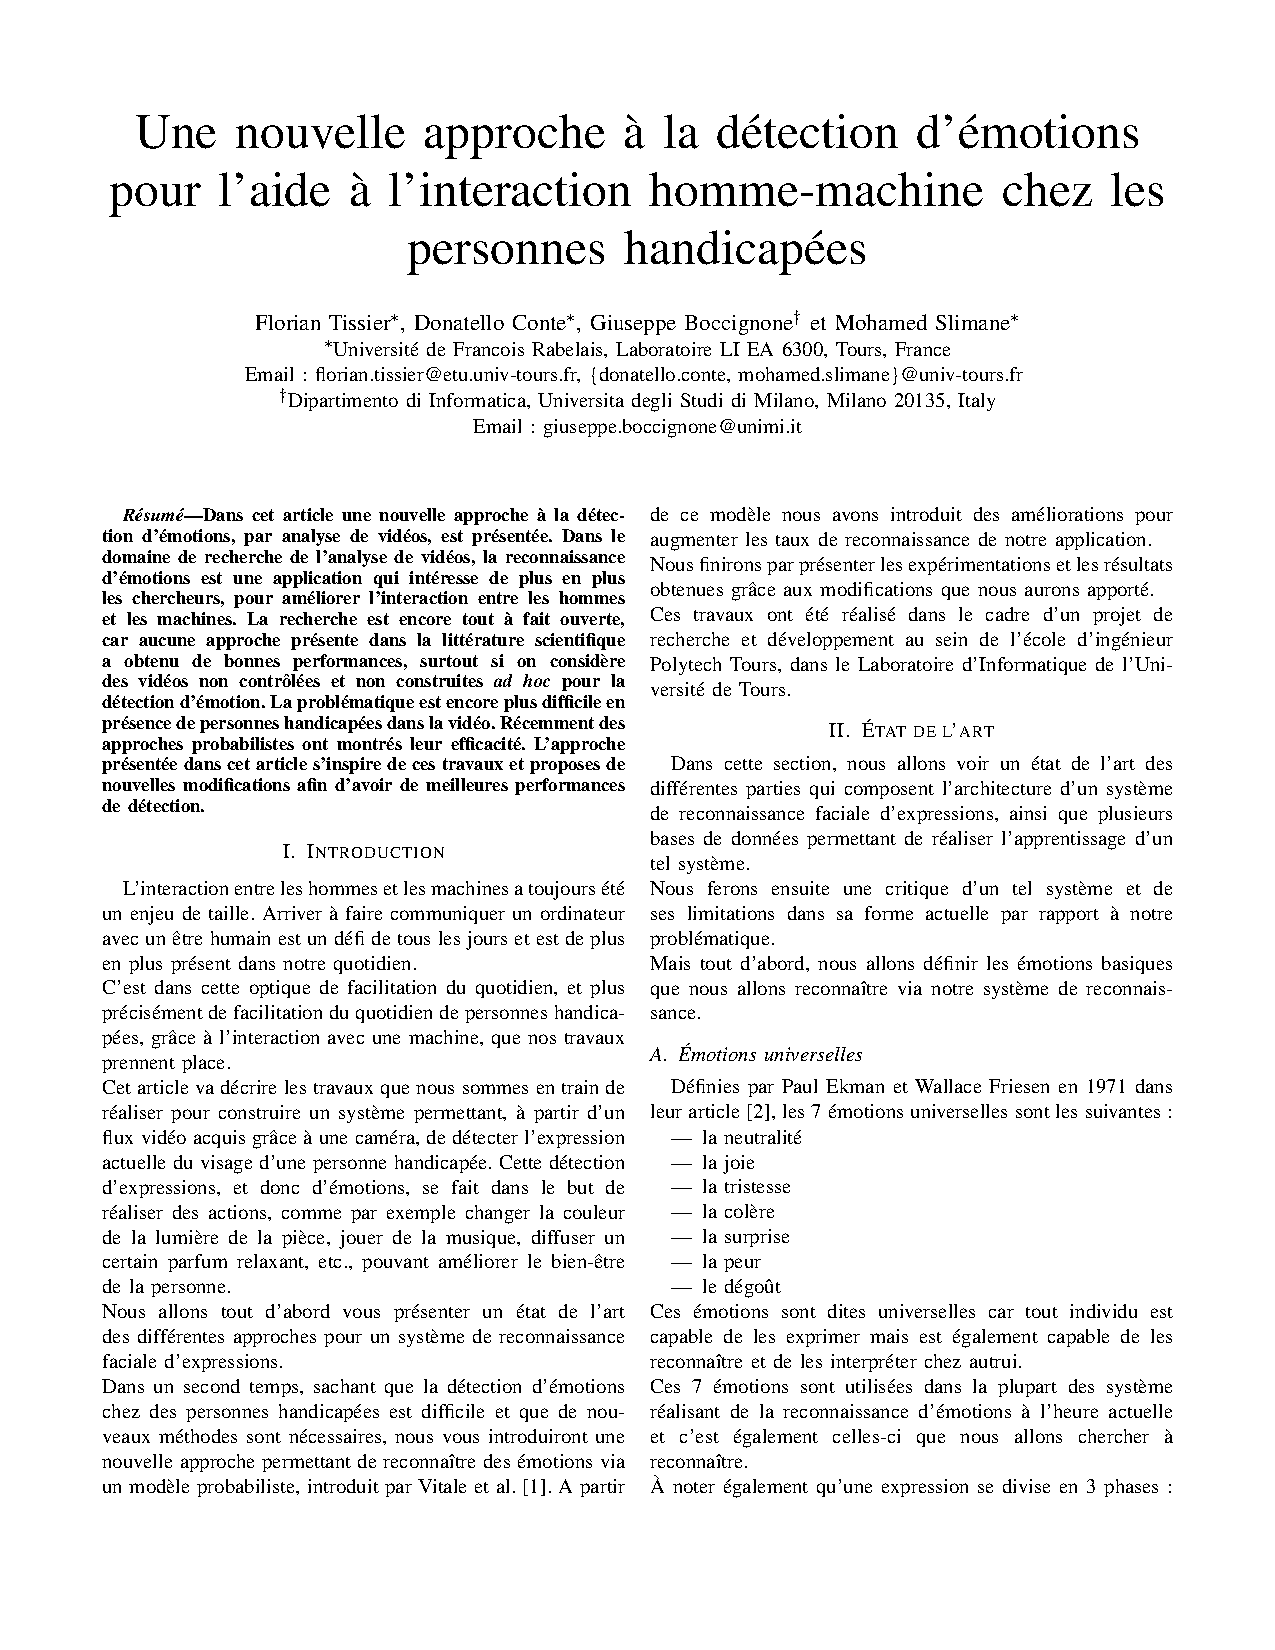
\includepdf[pages={1-6}]{images/une-nouvelle-approche.pdf}

\weeklyreport{17/09/2015}{
	Découverte de 2 grandes méthodes de description des mouvements du visage existent : le FACS (Facial Action Coding System) mis en place par P. Ekman et w. Friesen en 1978 et le FAPU (Facial Animation Parameter Units) introduit par la norme de codage vidéo MPEG-4.\\
	Recherche sur les types d'acquisitions d'images en 2D ou en 3D avec le matériel nécessaires à chaque fois ainsi que les algorithmes disponibles.
}
\weeklyreport{24/09/2015}{
	Recherche sur comment se décompose un bon système de reconnaissance facial d'émotions.\\
	Décomposition en 4 parties (récupération du visage, normalisation, extraction des points clés, classification) et recherche plus poussée sur les 2 premières parties.
}
\weeklyreport{01/10/2015}{
	Continuation des recherches sur les 2 dernières parties du système.\\
	Recherche également sur les différentes bases de données 2D publics disponibles à l'utilisation.
}
\weeklyreport{08/10/2015}{
	Recherche plus approfondies sur les filtres de Gabor. Présentation de mes recherches à Messieurs Conte et Slimane.\\
	Commencement de l'écriture du rapport.
}
\weeklyreport{15/10/2015}{
	Continuation des recherches sur les filtres de Gabor et leur fonctionnement. J'ai essayé de comprendre le fonctionnement des filtres et l'impact des différents paramètres. Grâce à un simulateur que j'ai trouvé en ligne (\cite{simu_gabor}) et aux instructions associées (\cite{instr_simu_gabor}), j'ai pu constater l'effet qu'ont les différents paramètres sur le résultat final.
}
\weeklyreport{22/10/2015}{
	Étude approfondi des bases de données MMI Mimicry et HCI Tagging.
}
\weeklyreport{05/11/2015}{
	Documentation sur les caractéristiques pseudo-Haar et leur fonctionnement.\\
	Recherche de techniques permettant de placer les points clés d'un visage sans FACS (ASM, AAM ...)
}
\weeklyreport{12/11/2015}{
	Réunion avec Mrs Conte et Slimane : décision de l'arrêt de la phase état de l'art pour commencer le développement; prise de décision sur les spécifications de notre système.\\
	Rédaction du rapport.	
}
\weeklyreport{19/11/2015}{
	Documentation plus poussée sur ASM, récupération d'un programme Matlab d'analyse d'émotions réalisé par des collègues italiens à Mr Conte et tentative de le faire fonctionner sous Octave vu que nous ne possédons pas de licence Matlab.\\
	Commencement de la prise en main de la librairie C++ OpenCV mais suite à un entretien avec Mr Conte, la décision a été prise de changer les spécifications de notre programme pour continuer le travail qui a déjà été réalisés par ses collègues italiens.
}
\weeklyreport{26/11/2015}{
	Étude approfondi de l'article écrit par Vitale et al. (\cite{italiens}) et rendez vous avec Mr Conte pour faire fonctionner le programme Matlab, presque fonctionnel au final.
}
\weeklyreport{03/12/2015}{
	Fin de l'étude approfondi de l'article de Vitale et al.\\
	Travail sur le programme Matlab pour le faire fonctionner à 100\%.
}
\weeklyreport{10/12/2015}{
	Rédaction du rapport.\\
	Téléchargement de Matlab pour faire fonctionner le programme car il est impossible de le faire fonctionner avec Octave.\\
	RDV avec Mr Conte pour vérifier la compréhension de l'article, des zones d'ombre persistent.
}
\weeklyreport{17/12/2015}{
	Étude du programme Matlab fonctionnel et comparaison de l'article au programme pour trouver à quelle partie du programme correspond chaque partie de l'article dans le but de mieux le comprendre.
}
\weeklyreport{Vacances de Noël}{
	Fin de rédaction du rapport 
}
\weeklyreport{07/01/2016}{
	Création du PowerPoint pour la soutenance et répétitions.\\
	Modification du programme Matlab pour qu'il prenne une image en entrée et l'affiche sur l'espace latent.\\
	Création nouvelle base d'apprentissage plus adaptée, avec des images plus grandes.
}
\weeklyreport{14/01/2016}{
	Soutenance de la partie Recherche\\
	Continuation de la création de la base d'apprentissage en réduisant la taille des images (les images étaient trop grandes et faisaient crasher mon ordinateur)
}
\weeklyreport{21/01/2016}{
	Rédaction d'un article scientifique sur les travaux réalisés lors de ce projet. L'article sera soumis à la conférence Handicap 2016. Rédaction de l'introduction à 90\%, de l'état de l'art à 15\% et de la méthode proposée à 100\%\\
	Au niveau du programme Matlab: 
	\begin{itemize}	
		\item création nouvelle base d'apprentissage: 31 images de taille 50*81 pixels
		\item prise d'une image en entrée
		\item association d'une émotion à une image
	\end{itemize}
Mais classification peu efficace pour l'instant.
}
\weeklyreport{28/01/2016}{
	Rédaction de l'article scientifique.\\
	Conférence Skype avec Giuseppe Boccignone pour nous aider dans nos travaux et nous donner de nouvelles pistes. Plusieurs améliorations ont été dégagés de cette conférence:
	\begin{itemize}
		\item changer la représentation des données, passer d'une représentation pixellique à une représentation vectorielle, ce qui nous permettrait de nous affranchir de l'algorithme PCa qui est très chronophage dès qu'une image est un peu grande
		\item changer la base d'apprentissage avec des images de grandes tailles
		\item représenter sur l'espace latent la trajectoire dans le temps d'une émotion plutôt que seulement la position d'une image
		\item utiliser l'algorithme FGPLVM (Faster GPLVM) plutôt que l'algorithme GPLVM utilisé précédemment
		\item migrer le programme de Matlab vers Python\\
	\end{itemize}
	Tentative de migration sous Python mais sans succès et donc prise en main du FGPLVM sous Matlab.
}
\weeklyreport{04/02/2016}{
	Fin de la rédaction de l'article scientifique.\\
	Création de la nouvelle base d'apprentissage (5 émotions * 15 frames) pour générer les trajectoires.
}
\weeklyreport{11/02/2016}{
	Soumission de l'article scientifique à la conférence Handicap 2016 \cite{handicap2016}.\\
	Recherche d'une détection des features avec Matlab pour utiliser la position de ces features comme données pour construire l'espace latent\\
	Création de l'espace latent avec toutes les trajectoires.
}
\weeklyreport{Vacances de Février}{
	Création de l'espace latent avec les coordonnées ou les distances des K plus proches voisins de chaque point (avec K=1,3,5,10).\\
	Traçage des trajectoires correspondantes sur l'espace latent.
}
\weeklyreport{25/02/2016}{
	Tentative d'ajouter sur l'espace latent des images passées en entrée représentant l'évolution d'une émotion: sans succès.
}
\weeklyreport{03/03/2016}{
	Envoi d'un mail à Giuseppe Boccignone pour lui demander des conseils et de l'aide.
	Rédaction de la partie Développement du rapport
}
\weeklyreport{10/03/2016}{
	Rédaction du rapport.\\
	Réception de la réponse de G. Boccignone, tentative d'application de ce qu'il a dit mais sans succès donc renvoi d'un second mail
}
\weeklyreport{17/03/2016}{
	Rédaction du rapport.\\
	Réception de la seconde réponse de G. Boccignone et ce coup-ci ses conseils nous ont permis d'afficher une trajectoire de test sur l'espace latent comme il faut.\\
	Recherche d'un algorithme permettant de comparer des trajectoires basé sur leurs formes.\\
	Création d'une base de test pour tester la précision de notre système.
}
\weeklyreport{24/03/2016}{
	Fin de rédaction du rapport.\\
	Préparation de la soutenance.
}


\makelastpages

\end{document}


